\documentclass[12pt,a4paper,onecolumn,oneside,titlepage]{article}
\usepackage[utf8]{inputenc}
\usepackage[german]{babel}

\usepackage[T1]{fontenc}
\usepackage{amsmath}
\usepackage{amsfonts}
\usepackage{amssymb}
\usepackage{tikz}

\usepackage{footnote}
\makesavenoteenv{tabular}
\usepackage{wrapfig}
%for pseudocode
\usepackage{algorithm}
\usepackage{algpseudocode}
\usepackage{caption}
\usepackage{subcaption}
\usepackage{url}
\usepackage{booktabs}



\DeclareCaptionFormat{algor}{%
  \hrulefill\par\offinterlineskip\vskip1pt%
    \textbf{#1#2}#3\offinterlineskip\hrulefill}
\DeclareCaptionStyle{algori}{singlelinecheck=off,format=algor,labelsep=space}
\captionsetup[algorithm]{style=algori}


%return on a new line
\let\oldReturn\Return
\renewcommand{\Return}{\State\oldReturn}

\newcommand{\vars}{\texttt}
\newcommand{\func}{\textsc}
\newcommand\cursive[1]{\ensuremath{\mathcal{#1}}}

\makeatletter
\renewcommand{\ALG@name}{Algorithmus}
\makeatother

\setcounter{tocdepth}{2}

\author{}
\title{}
\makeindex
\begin{document}

  \begin{titlepage}
   \centering
    \vspace{5cm}
    {\scshape\huge Heuristiken für das Entfernen von verbotenen Teilgraphen\par}
      \vspace{1cm}
    {\large\bf Paul Walger (349968)}\\
      \vspace{1cm}
    {\large\ 5. Juli 2016}\\
      \vspace{1cm}
    {\large\ Technische Universität Berlin, Fakultät IV \\ Algorithmik und Komplexitätstheorie}\\
      \vspace{3cm}
      

\begin{tabular}{l  l}
\textbf{Gutachter:} & Prof. Dr. Rolf Niedermeier \\
 & Prof. Dr. Stephan Kreutzer \\\\
\textbf{Betreuer:} & Dr. Falk Hüffner \\
 & Dr. Christian Komusiewicz 
\end{tabular} 


      \vspace{1cm}
      
    \newpage
    
    
     \begin{quote}
        \textbf{Zusammenfassung:}\\ Graphen so zu modifizieren, dass sie gewisse induzierte Teilgraphen nicht mehr enthalten, ist bis auf gewisse triviale Fälle NP-vollständig. Dieses Problem ist unter dem Namen \textsc{\cursive{F}-Free Edge Editing} bekannt und hat als Eingabe einen Graphen und eine Menge von verbotenen Graphen. 
Für einige Mengen von verbotenen Teilgraphen wurde bereits gute Heuristiken entwickelt. In dieser Arbeit werden Heuristiken für die Lösung des Problemes erarbeitet, indem drei verschiedene Ansätze entwickelt werden, welche \textsc{\cursive{F}-Free Edge Editing} für beliebige \cursive{F} lösen. Diese werden auf ihre Güte und Geschwindigkeit auf zufälligen und realen Datensätzen von Graphen getestet. Dafür wurde \textsc{\cursive{F}-Free Edge Editing} mittels Binary-Integer-Programming gelöst, um optimale Lösungen zu bestimmen. Außerdem werden diese allgemeinen Heuristiken mit spezifischen Heuristiken verglichen.
    \end{quote}
    \vspace{2cm}
    \begin{quote}
          \textbf{Abstract:}\\ To modify graphs in such a way, that they will not contain certain induced subgraphs is mostly NP-complete. This problem is known as \textsc{\cursive{F}-Free Edge Editing} and gets a graph and a set of forbidden graphs and answers with the minimal amount of changes required, so that the graph will not contain the forbidden subgraphs.
          For certain sets auf \cursive{F} good heuristics already exists. But in this paper, we will develop 3 different heuristics for general sets of forbidden subgraphs. We will test the quality and performance of the heuristics. To make this possible, we solved \textsc{\cursive{F}-Free Edge Editing}  using binary integer programming to obtain optimal solutions. We also compare our general heuristics to other specific heuristics.
    \end{quote}
    
  \end{titlepage}
\newpage
\textbf{Eidesstattliche Erklärung}\\\\
Hiermit erkläre ich, dass ich die vorliegende Arbeit selbstständig und eigenhändig sowie ohne
unerlaubte fremde Hilfe und ausschließlich unter Verwendung der aufgeführten Quellen und Hilfsmittel
angefertigt habe.\\\\
Berlin, den \\\\
…………………………………………………………………\\\\
Unterschrift\\
\newpage
\tableofcontents
\newpage 
\section{Einleitung}

Graphen sind eine bildliche Darstellung von Beziehungen zwischen Objekten. Damit können sie eine Vielzahl von Problemen und Szenarien modellieren \cite{Nastos06}.

\subsection{Motivation}
\label{sec:mot}
Wird nun ein System von Objekten mittels einem Graphen modelliert, hat der Graph ebenso wie das modellierte System gewisse charakteristische Eigenschaften.

Eine solche Eigenschaft wäre, dass wenn ein beliebiger Knoten im Graphen $u$ mit einem anderen Knoten $v$ verbunden ist, so ist $u$ auch mit allen Nachbarn von $v$ verbunden. Graphen mit dieser Eigenschaft werden Cluster-Graphen  genannt. Diese bestehen aus einer oder mehreren Komponenten, in welcher jeder Knoten mit jedem Knoten verbunden ist.
Diese Cluster-Graphen lassen sich aber auch dadurch charakterisieren, dass sie gewisse Strukturen nicht besitzen und zwar, dass sie nicht den Graphen $P_3$ als einen induzierten Teilgraphen haben. Der $P_3$ Graph ist in der Abbildung \ref{fig:mot-p3} zu sehen.
Einen $P_3$ als induzierten Teilgraphen zu haben bedeutet, dass man jedem Knoten aus dem $P_3$ einen Knoten aus dem Graphen zuordnen kann, sodass gilt, dass wenn zwei Knoten im $P_3$ durch eine Kante verbunden sind, so sind auch die entsprechenden Knoten in dem Graphen durch eine Kante verbunden. Und umgekehrt, dass wenn zwei Knoten im Graphen verbunden sind, so sind auch die Knoten im $P_3$ verbunden.
 
Erklären lässt sich das an der Abbildung \ref{fig:mot}.
In dem Graphen $G_1$ in der Abbildung \ref{fig:mot-1} sehen wir, dass der Teilgraph mit den Knoten B,D und C ein vom $P_3$ induzierter Teilgraph ist, weil wir den Knoten $a$ aus dem $P_3$ Graphen dem Knoten $B$ im Graphen $G_1$, den Knoten $b$ dem Knoten $C$ und den Knoten $c$ dem Knoten $D$ zuordnen können, sodass die vorhin geforderte Eigenschaft gilt.
So sehen wir, dass im Graphen $P_3$ die Knoten $a$ und $c$ verbunden sind und im  
$G_1$ auch die Knoten $B$ und $D$ verbunden ist. Auch ist $B$ und $C$ in Graphen $G_1$ nicht verbunden und $a$ und $b$ im $P_3$ Graphen ebenso.  Man kann überprüfen, dass die Voraussetzung für jedes beliebige Paar von Knoten geben ist und so ist der fett markierte Teilgraph in $G_1$ ein von $P_3$ induzierter Teilgraph. 

Der Graph $G_2$ in der Abbildung \ref{fig:mot-2} hat keinen $P_3$ als induzierten Teilgraphen, weil wir nicht die Knoten vom $P_3$ zu Knoten in diesem Graphen zuordnen können und dabei unsere Voraussetzung erfüllt bleibt. Wenn wir also zum Beispiel die Zuordnung vom Knoten $a$ zum Knoten $A$, $b$ zu $B$ und $c$ zu $C$ nehmen, sehen wir das Problem, dass wir eine Kante zwischen $A$ und $C$ haben, aber keine Kante zwischen $a$ und $b$. Somit ist das keine gültige Zuordnung. Man kann aber auch nachvollziehen, dass egal wie die Zuordnung gewählt wird, es nicht möglich ist, die vorhin geforderte Eigenschaft zu erfüllen.

\begin{figure}
  \centering
 
  \begin{tabular}[c]{ccc}
    \begin{subfigure}[b]{0.32\textwidth}
      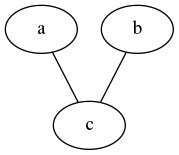
\includegraphics[scale=0.6]{dot/dot_mot_p3.png}
   
      \caption{Ein $P_3$ Graph }
      \label{fig:mot-p3}
   \end{subfigure}&
	 \begin{subfigure}[b]{0.32\textwidth}
	 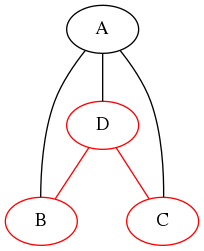
\includegraphics[scale=0.5]{dot/dot_mot_1.png}
	 
	    \caption{Graph $G_1$ mit einem von $P_3$ induzierten Teilgraphen.}
	    \label{fig:mot-1}
	  \end{subfigure}&
    \begin{subfigure}[b]{0.32\textwidth}
       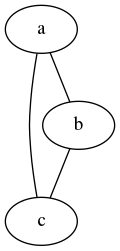
\includegraphics[scale=0.5]{dot/dot_mot_2.png}
	    \caption{Graph $G_2$ ohne einen induzierten $P_3$}
	    \label{fig:mot-2}
    \end{subfigure}
  \end{tabular}
  \caption{Cluster-Graphen}\label{fig:mot}
\end{figure}

Deshalb ist der Graph $G_2$ ein Cluster-Graph und hat eben diese besondere Eigenschaft, die auf zwei Weisen beschrieben werden kann: 
\begin{itemize}
 \item der Graph hat eine oder mehrere Komponenten wo jeder Knoten mit jedem Knoten verbunden ist
 \item der Graph hat kein $P_3$ als einen induzierten Teilgraphen
\end{itemize}
Die erste Charakterisierung ist eine mehr natürliche und wir könnten zu einer solchen Beschreibung aus praktischen Beobachtungen über unsere Daten kommen, während die zweite eine eher mathematische ist und nicht immer intuitiv, aber dennoch sehr nützlich ist, weil wir eine Eigenschaft klar formulieren können.

In dieser Arbeit werden wir uns Methoden erarbeiten, welche einen Graphen so modifizieren, sodass er bestimmte Eigenschaften hat und zwar Eigenschaften, welche sich mittels einer Charakterisation durch verbotene Teilgraphen beschreiben lassen.

\subsection{Definitionen}
\subsubsection{Notationen}
\label{sec:notation}
Mit Graphen sei im Folgenden stets ein ungerichteter, einfacher Graph gemeint. Wenn nicht anders angegeben ist, ist $G=(V,E)$ ein Graph, $V$ die Menge seiner Knoten und $E$ die Menge seiner Kanten.

Die Menge der Knoten des Graphen $G$ ist $V(G)$ und die Menge der Kanten des Graphen $G$ heißt $E(G)$. Die Nachbarschaft von dem Knoten $u$ heißt $N(u)$, während $N^{*}(u)$ die Nachbarschaft von $u$ inklusive $u$ ist. Ein Pfad der Länge $i$ wird als $P_i$ bezeichnet. Ein Kreis der Länge $i$ wird als $C_i$ bezeichnet.

Eine Kante $k$ in einem Graphen $G$ zu kippen (oder auf engl. flip) heißt, dass man die Kante aus dem Graphen $G$ entfernt, wenn $k \in E(G)$ oder, dass man die Kante $k$ in der Graphen $G$ einfügt, wenn $k \notin E(G)$.
 
Sei $G = (V,E)$ ein Graph und $S \subseteq V$ eine beliebige Knotenteilmenge von $V$. 
Dann ist $G[S] = (S, E \cap \{\{u,v\} \,|\, u \in S \land w \in S\})$ der durch $S$ induzierte Teilgraph von $G$. Die Degeneracy eines Graphen $G$ ist das kleinste $k \in \mathcal{N}$, sodass jeder induzierte Teilgraph von $G$ einen Knoten mit $k$ oder weniger Nachbarn hat.

Seien $H = (V_H,E_H)$ und $G =(V,E)$ zwei Graphen. Ein Subgraph-Isomorphismus von H nach G ist eine Funktion $f : V_H \rightarrow V$, sodass $(u,v) \in E_H $ gilt, genau dann wenn $(f(u),f(v)) \in E$.

Seien $G$ und $F$ Graphen, dann ist der Graph $G$ \textit{F}-frei, wenn es nicht \textit{F} als induzierten Teilgraph enthält. Für eine Menge \cursive{F} von Graphen, heißt der Graph $G$ \cursive{F}-frei, wenn $G$ \textit{F}-frei ist für jeden \textit{F} $\in \cursive{F}$. Ein Graph heißt valide, wenn er \cursive{F}-frei ist. 

Die Kantendifferenz  $\delta(G_1,G_2) = E(G_1) \Delta E(G_2)$ zwischen zwei Graphen $G_1$ und $G_2$ ist definiert als die symmetrische Differenz der Kantenmengen der beiden Graphen\footnote{Dies ist möglich, weil wir nur Graphen vergleichen, die die selben Knoten haben}. Die Editierdistanz zwischen zwei Graphen definieren wir hier als $\Delta(G_1,G_2) = |\delta(G_1,G_2)|$.
Die normierte Editierdistanz $\delta^{*}(G_1,G_2)$ zwischen zwei Graphen $G_1$ und $G_2$ ist  $\Delta^{*}(G_1,G_2) =  \frac{\Delta(G_1,G_2)}{|E(G_2)|^2}$.

Ein ungerichteter Graph $G$ heißt Wald, wenn er keinen Zyklus enthält. Ist der Graph $G$ zudem zusammenhängend, dann heißt er auch Baum. Jede Zusammenhangskomponente eines Waldes ist daher ein Baum.

In Tabelle \ref{tab:graph_charac} sind die in dieser Arbeit erwähnten Graphen-Klassen mit ihren Charakterisationen durch verbotene Teilgraphen aufgelistet.


\begin{table}

\centering

\begin{tabular}{c c}
\textbf{Graphklasse} & \textbf{Charakterisation}\\ 
\hline 
Threshold & $P_4, C_4, \overline{C_4}$ \\
Cograph & $P_4$ \\
Cluster & $P_3$  \\
Split & $C_4, C_5, \overline{C_4}$ \\
Splitcluster & $C_4$,$C_5$,$P_5$, Bowtie, Necktie \\
Quasi-Threshold & $P_4,C_4$ \\
Claw-Free & $K_{1,3}$

\end{tabular} 
\caption{Charakterisation einiger Graphenklassen durch verbotene Teilgraphen}
\label{tab:graph_charac}
\end{table}


\subsubsection{Problemstellung}
\label{sec:problem}
Das Problem, für das in dieser Arbeit Heuristiken entwickelt werden, kann wie folgt definiert werden:
\begin{quote}
  \textsc{\cursive{F}-Free Edge Editing}\newline
  \textbf{Eingabe:} Graph $G$, natürliche Zahl $k$, Menge von Graphen \cursive{F}\newline
  \textbf{Frage:} Können wir in $G$ höchstens $k$ Änderungen machen, sodass $G$ keinen induzierten Teilgraphen aus \cursive{F} enthält?\newline
  \textbf{Parameter:} $k$
\end{quote}
In dieser Arbeit werden wir uns darauf beschränken, dass \cursive{F} eine endliche Menge ist. Dabei ist jeder Graph in \cursive{F} kein kantenloser Graph ist.
Des weiteren gibt es das \textsc{F-Free Edge Editing}, wo \textsc{F} keine Menge von Graphen, sondern nur ein Graph ist. \\


\textbf{Ähnliche Probleme:}

\begin{quote}
  \textsc{\cursive{F}-Free Edge Deletion/Completion}\newline
  \textbf{Eingabe:} Graph $G$, natürliche Zahl $k$, Menge von Graphen \cursive{F}\newline
  \textbf{Frage:} Können wir in $G$ höchstens $k$ Kanten löschen/entfernen  machen, sodass $G$ keinen induzierten Teilgraphen aus \cursive{F} enthält?\newline
  \textbf{Parameter:} $k$
\end{quote}

\begin{quote}
  \textsc{\cursive{F}-Free Vertex Deletion/Completion}\newline
  \textbf{Eingabe:} Graph $G$, natürliche Zahl $k$, Menge von Graphen \cursive{F}\newline
  \textbf{Frage:} Können wir in $G$ höchstens $k$ Knoten löschen/entfernen  machen, sodass $G$ keinen induzierten Teilgraphen aus \cursive{F} enthält?\newline
  \textbf{Parameter:} $k$
\end{quote}

\subsection{Anwendungsbeispiele}
\label{sec:examples}
In diesem Abschnitt werden auf einige Anwendungsfälle eingegangen, warum Graphen mit bestimmten Eigenschaften gewünscht sind.

\newpage
\subsubsection{Soziale Netzwerke}
 
\begin{wrapfigure}{r}{0.4\textwidth}
  \begin{center}
    
\begin{tikzpicture}
  [shorten >=2pt,node distance=1cm,auto,main node/.style={circle,draw,align=center}]
  \node[main node, fill=gray] (a) at (4,10) {};
\node[main node] (b) at (3,9)  {};
\node[main node] (c) at (5,9)  {};
\node[main node] (d) at (2,8) {};
\node[main node] (e) at (4,8)  {};
\node[main node] (g) at (6,8)  {};
  
\node[main node] (f) at (2,7)  {};
  
  
  \draw (a) -- (b);
  \draw (a) -- (c);
  \draw (b) -- (d);
  \draw (b) -- (e);
  \draw (d) -- (f);
  
  \draw (c) -- (g);
  
  \path
(a) edge [bend left=35,dashed] node {} (g)
    edge [bend left=30,dashed] node {} (f)
    edge [bend right=35,dashed] node {} (d)
    edge [bend left=10,dashed] node {} (e)
(b) edge [bend left=15,dashed] node {} (f);


\end{tikzpicture}


  \end{center}
  \caption{Ein Quasi-Threshold Graph}
  \label{fig:quasi-threhold}
\end{wrapfigure}
Eine familiäre Struktur oder eine Gemeinschaft, die hierarchisch organisiert ist, wird durch $(P_4,C_4)$-freie Graphen modelliert. Diese Graphen werden auch trivial perfekte Graphen oder Quasi-Threshold Graphen genannt \cite{Wolk65}. 

Die letztere Bezeichnung kommt von der Charakterisierung dieser Graphen als baumartige Strukturen. Ein solcher gerichteter Graph lässt sich als der transitive Abschluss eines Waldes sehen \cite{BrandesHSW15}. Dieser Graph muss gerichtet sein, weil es sonst eine Clique wird.

In der Abbildung \ref{fig:quasi-threhold} ist  ein Quasi-Threshold Graph zu sehen. Die durchgehenden Kanten zeigen den Wald, in diesem Fall ist es ein Wald mit genau einem Baum. Der dunkle-graue Knoten ist die Wurzel des Baumes.  Dabei stellen gestrichelten Kanten den transitiven Abschluss dar.
Solche Graphen modellieren eine große Anzahl von Netzwerken. Unter anderem auch soziale Strukturen, wie eine Hierarchie in einer Organisation. Dabei modellieren die Knoten Personen und die Kanten stellen die Wege dar, auf denen die Befehle fließen. Fast alle haben einen Vorgesetzten (bis auf die Wurzel) und nehmen Befehle von dem Vorgesetzten an, was durch die Baumstruktur modelliert wird. Aber sie hören auch auf die Befehle von dem Vorgesetzen des Vorgesetzen, was durch den transitiven Abschluss modelliert wird\cite{NastosG13}. 

Ähnlich dazu sind $(P_5,C_5)$-freie Graphen die auch soziale Strukturen modellieren und dafür geeignet sind Gemeinschaften zu identifizieren \cite{Schoch15}. 

\subsubsection{\textsc{Maximum Clique} auf Co-Graphen}
Um das Problem der \textsc{Maximum Clique}, welches die größte Clique in einem Graphen findet, auf einem Graphen $G$ zu lösen, kann man wie folgt vorgehen. Es ist offensichtlich, dass wenn der Graph zwei Zusammenhangskomponenten hat, dass es dann möglich ist \textsc{Maximum Clique} auf den beiden Komponenten lösen und das Maximum davon ist das Resultat für den Graphen $G$. Somit kann das Problem also in kleinere Probleme zerlegt werden.
Außerdem gilt es, dass das Finden einer Clique in einem Graphen $G$ äquivalent zum Finden einer stabilen Menge in dem Komplementgraphen von $G$ ist.
Es ist also möglich, das Problem weiter zu zerlegen, indem das Komplement von jeder Zusammenhangskomponente genommen wird und es wieder in seine Zusammenhangskomponenten zerlegt wird. Dabei gilt, dass eine maximale stabile Menge die Vereinigung aller maximalen stabilen Mengen der Zusammenhangskomponente ist \cite{Nastos06}. 

Eine solche Vorgehensweise ist offensichtlich sehr attraktiv um ein schweres Problem, wie \textsc{Maximum Clique} es ist, zu lösen. Dieses Vorgehen kommt jedoch in eine Sackgasse, wenn der Komplementgraphen nicht mehr zerlegt werden kann, weil er keine Zusammenhangskomponenten mehr hat.
Dann funktioniert diese Vorgehensweise nicht mehr. 

Aber es gibt eine Klasse von Graphen, die \glqq complement reducible graphs \grqq oder kurz Co-Graphen, die so definiert worden ist, dass es nicht zu dem eben beschriebenen Sackgasse nicht kommen kann.
Das bedeutet, dass \textsc{Maximum Clique} in linearer Zeit auf solchen Graphen lösbar ist, während auf allgemeinen Graphen \textsc{Maximum Clique} NP-vollständig ist.
Diese Klasse von Co-Graphen ist auch durch charakterisiert, dass sie keinen $P_4$ als induzierten Teilgraphen enthalten \cite{NastosG13}.


\subsubsection{Protein-Interaktionsnetzwerke}


\begin{figure}
  \centering
  \begin{tabular}[c]{cccc}
    \begin{subfigure}[b]{0.32\textwidth}
     \begin{tikzpicture}
      [shorten >=2pt,node distance=1cm,auto,main node/.style={circle,draw,align=center}]
        \node[main node] (a) at (2.5,1.75) {};
        \node[main node] (b) at (1.5,1)  {};
        \node[main node] (c) at (3.5,1)  {};
        \node[main node] (d) at (2,0) {};
        \node[main node] (e) at (3,0)  {};
  
  
        \draw (a) -- (b);
        \draw (a) -- (c);
        \draw (b) -- (d);
        \draw (d) -- (e);
        \draw (e) -- (c);

      \end{tikzpicture}  
      \caption{$C_5$}
      \label{fig:graphs:c5}
    \end{subfigure}&
    \begin{subfigure}[b]{0.32\textwidth}
      \begin{tikzpicture}
      [shorten >=2pt,node distance=1cm,auto,main node/.style={circle,draw,align=center}]
        \node[main node] (a) at (1,2) {};
        \node[main node] (b) at (2,2)  {};
        \node[main node] (c) at (1,1)  {};
        \node[main node] (d) at (2,1) {};
  
  
        \draw (a) -- (b);
        \draw (a) -- (c);
        \draw (b) -- (d);
        \draw (d) -- (c);

      \end{tikzpicture}  
      \caption{$C_4$}
      \label{fig:graphs:c4}
    \end{subfigure}&
    \begin{subfigure}[b]{0.32\textwidth}
     \begin{tikzpicture}
      [shorten >=2pt,node distance=1cm,auto,main node/.style={circle,draw,align=center}]
        \node[main node] (a) at (1,2) {};
        \node[main node] (b) at (2,2)  {};
        \node[main node] (c) at (1,1)  {};
        \node[main node] (d) at (2,1) {};
  
  
        \draw (a) -- (c);
        \draw (b) -- (d);

      \end{tikzpicture}  
      \caption{$2K_2$}
      \label{fig:graphs:2k2}
    \end{subfigure}
  \end{tabular}
  \caption{Die verbotenen Graphen in einem Split-Graphen}\label{fig:split_graphs}
\end{figure}
In dem Abschnitt \ref{sec:mot} haben wir Cluster-Graphen betrachtet, wo jede Zusammenhangkomponente eine Clique ist.
Split-Graphen sind ähnliche Graphen, aber bestehen nur aus einer Clique und einigen Knoten, die an der Clique anhängen. Formell definiert heißt es, dass man die Menge der Knoten des Graphen in zwei Mengen $V_1$ und $V_2$ teilen kann, sodass G[$V_1$] ein stabile Menge und G[$V_2$] eine Clique ist. Split-Graphen lassen sich als $(2K_2, C_4, C_5)$-freie Graphen beschrieben. 
Dazu ist ein Splitcluster-Graph ein Graph wo jede Zusammenhangkomponente ein Split-Graph ist \cite{BrucknerHK15}.

Diese Struktur modelliert gut Protein-Protein-Interaktionsnetzwerke. In Körper vom Menschen oder anderen Lebewesen gibt es eine Vielzahl von Proteinen, die einen Zweck haben, aber diesen erfüllen sie meistens nicht alleine, sondern in dem sie Proteinkomplexe bilden. Diese Proteinkomplexe bestehen aus einer großen Anzahl von Proteinen und sind nicht einfach zu untersuchen. Ein Weg um solche Proteinkomplexe zu identifizieren besteht darin, herauszufinden welche Proteine mit welche Proteinen überhaupt interagiert. So kann man diese Proteine als Knoten ansehen und wenn es eine Interaktion zwischen diesen Proteinen gibt, diese als eine Kante ansehen. 
Ein Proteinkomplex hat einen Kern, wo jedes Protein mit jedem Protein interagiert und Anhängsel, einzelne Proteine, die nur mit dem Kern interagieren. Damit modellieren Splitcluster-Graphen die Struktur von Proteinkomplexen und können dazu verwendet werden um Proteinkomplexe zu bestimmen\cite{BrucknerHK15}.

\subsection{Annäherung}
Jedoch haben die Eingabedaten typischerweise Fehler oder sind unvollständig. So können in einem Cluster-Graphen bestimmte Kanten fehlen, obwohl sie dazu gehören sollten. Oder in Splitcluster-Graphen fehlen Informationen zu Interaktionen von gewissen Paaren von Proteinen. Weil die Daten nun fehlerhaft sind, stellt sich die Frage, wie viele und welche Änderung müssen am Graphen getan werden, damit der Graph die erwünschte Struktur hat. Wenn man nun die Struktur durch eine Menge \cursive{F} von verbotenen Graphen charakterisiert, nennt sich das Problem \textsc{\cursive{F}-Free Edge Editing}.

Nun ist \textsc{\cursive{F}-Free Edge Editing} für die meisten \cursive{F} sehr aufwendig zu lösen \cite{Burzyn06}, weil es NP-vollständig ist. 
Deswegen ist es attraktiv dieses Problem nicht optimal zu lösen, indem die minimale Anzahl von Änderungen gefunden wird, sonder einfach eine möglichst kleine Anzahl von Änderungen.

Was bringt es aber, wenn man nur eine Annäherung hat?  Vorallem soll es die Frage klären, wie gut eine allgemeine Heuristik ist, im Vergleich zu den auf spezifische Anwendungsfälle zugeschnittenen Heuristiken. Lohnt es sich überhaupt für spezifische \cursive{F} Heuristiken zu entwickeln? Oder können allgemeine Heuristiken eine guten Dienst leisten? 

\subsection{Ähnliche Arbeiten}
\subsubsection{Komplexität von \textsc{\cursive{F}-Free}}
Einige Edge Editing/Deletion/Completion Probleme wurde in \cite{Natanzon01} untersucht. Weitere Resultate zur der Komplexität wurden in \cite{Burzyn06} erbracht.
Einige von den Ergebnissen sind in der Tabelle \ref{tab:hardness} dargestellt. 

\begin{table}

\centering

\begin{tabular}{c ccc}
\textbf{Graphklasse} & \textbf{Edge Completion} & \textbf{Edge Deletion} & \textbf{Edge Editing} \\ 
\hline 
Threshold & NPC & NPC & ? \\
Cograph & NPC & NPC & NPC \\
Cluster & P & NPC & NPC \\
Split & NPC & NPC & P \\
Quasi-Threshold & NPC & NPC & ? \\
Triangle-Free & P & NPC & NPC \\
\end{tabular} 
\caption{Komplexitäts-Ergebnisse für einige Graphenklassen. Dabei steht NPC für ein NP-vollständiges Problem, P für ein polynomiales Problem und ? für ein offenes Problem.}
\label{tab:hardness}
\end{table}


Für \textsc{F-Free Edge Editing}, \textsc{F-Free Edge Completion} und \textsc{F-Free Edge Deletion} hat \cite{AravindSS15} folgende Ergebnisse gefunden:
\begin{itemize}
 \item \textsc{F-Free Edge Deletion} ist in polynomieller Zeit lösbar, wenn F ein Graph mit höchstens einer Kante ist.
 \item \textsc{F-Free Edge Completion} ist in polynomieller Zeit lösbar, wenn F ein Graph mit höchstens einer Nicht-Kante ist.
 \item \textsc{F-Free Edge Editing} ist in polynomieller Zeit lösbar, wenn F ein Graph mit höchstens zwei Knoten ist.
\end{itemize}
Bezüglich der NP-Vollständigkeit hat es folgende Ergebnisse:
\begin{itemize}
 \item \textsc{F-Free Edge Deletion} ist genau dann NP-vollständig, wenn F ein Graph mit mindestens zwei Kanten ist.
 \item \textsc{F-Free Edge Completion} ist genau dann NP-vollständig, wenn F ein Graph mit mindestens zwei Nicht-Kanten ist.
 \item \textsc{F-Free Edge Editing} ist genau dann NP-vollständig, wenn F ein Graph mit mindestens drei Knoten ist.
\end{itemize}
Ähnliche Fragen sind für \textsc{\cursive{F}-Free Edge Deletion/Completion/Editing} noch offen \cite{AravindSS15}.

\subsubsection{Approximationen}
Nach \cite{Cai96} gibt es für \textsc{\cursive{F}-Free Edge Editing} parametrisierbare Algorithmen. Jedoch gibt es nach \cite{Kratsch13} für die meisten \cursive{F} keine polynomiale Kernel für \textsc{\cursive{F}-Free Edge Editing}.

\subsubsection{Hitting-Set}
Es wurden Greedy-Alogrithmen für das Hitting-Set Problem entwickelt \cite{Moreno13}, welches sich wie folgt definieren lässt \cite{Karp72}: Gegeben ist ein Universum $U$ und eine Menge $\Gamma$ von Teilmengen von $U$. Gesucht ist eine Teilmenge $H$ von $U$, sodass jede Menge in $\Gamma$ ein Element aus $H$ enthält, dazu soll die Mächtigkeit der Menge kleiner sein als eine positive ganze Zahl $k$.

Wenn die Menge \cursive{F} endlich ist, dann kann das \textsc{\cursive{F}-Free Vertex Deletion} Problem leicht als \textsc{$d$-Hitting Set} formuliert werden, wobei die Konstante $d$ die größte Anzahl von Knoten in einem Graphen in \cursive{F} ist \cite{Kratsch13}. Damit gäbe es polynomiale Kernel für \textsc{\cursive{F}-Free Vertex Deletion} nach \cite{Abu10}.
Nach \cite{Bodlaender06} ist es offen, ob es für \textsc{F-Free Edge Deletion} analog auch polynomiale Kernel gibt.

Es scheint eine Ähnlichkeit zu dem \textsc{F-Free Edge Editing} zu bestehen, aber leider lässt sich das \textsc{F-Free Edge Editing} nicht leicht als ein Hitting-Set-Problem formulieren. Die Schwierigkeit beim Editing Problem ist, dass auch Kanten hinzugefügt werden können. Wenn wir nun das Universum $U$ als alle möglichen Kanten nehmen und $\Gamma$ die Menge der verbotenen Teilgraphen ist, dann wäre zwar $H$ die Menge der Änderungen, doch diese Änderungen könnten neue verbotene Teilgraphen erzeugen und somit den erzeugten Graphen nicht mehr F-frei machen.



\subsection{Überblick}
Im Kapitel \ref{sec:algos} werden die Algorithmen für die Heuristiken vorgestellt. Dann werden wir im Kapitel \ref{sec:tests} betrachten wie die Experimente aussehen und auf welchen Modellen diese Algorithmen auf ihre Güte getestet wurden und wie die Details der Implementierung aussehen.
Darauf folgend werden im Kapitel \ref{sec:results} die Resultate vorgestellt,  diskutiert und mit anderen Heuristiken verglichen werden.
\newpage 
\section{Algorithmen}

\label{sec:algos}

In diesem Abschnitt werden die verschiedenen Heuristik-Ansätze für \textsc{\cursive{F}-Free Edge Editing} vorgestellt. 
Die im nachfolgenden beschriebenen Algorithmen basieren alle auf dem folgenden Prinzip: Suche einen validen Graphen, welcher die verbotenen Teilgraphen nicht enthält. Wiederhole dies mehrmals und gebe dann die Differenz zwischen dem besten validen Graphen und dem Eingabegraphen aus.

Dieses Prinzip ist im Algorithmus \ref{algo:general} zu sehen. Dort ist \vars{$G_{input}$} der Eingabegraph, \cursive{F} die Menge der verbotenen Teilgraphen und \vars{$i_{max}$} die Angabe wie oft der Algorithmus wiederholt werden soll. Dabei steht \func{SolveAlgo} für einen der Algorithmen, die in den folgenden Abschnitten vorgestellt werden.
\begin{algorithm}
  \captionof{algorithm}{Genereller Aufbau}\label{algo:general}
\begin{algorithmic}[1]
\Function{Solve}{\vars{$G_{input}$}, \cursive{F}, \vars{$i_{max}$}}

\State{\vars{$G_{best}$} $\gets$ $(\emptyset,\emptyset)$}

\For{\vars{i} = 1 to \vars{$i_{max}$}}
	\State{\vars{$G_{valid}$} $\gets$ \func{solveAlgo}(\vars{$G_{input}$}, \cursive{F})}
	\If{$\Delta$(\vars{$G_{input}$}, \vars{$G_{best}$}) < $\Delta$(\vars{$G_{input}$}, \vars{$G_{valid}$})|}
		\State{\vars{$G_{best}$} $\gets$ \vars{$G_{valid}$}}
	\EndIf  
\EndFor

\Return{$\delta$(\vars{$G_{input}$}, \vars{$G_{best}$})}
\EndFunction
\end{algorithmic}
\end{algorithm}

Da alle Ansätze diese Schritte enthalten und sich nur darin unterschieden, wie der valide Graph mittels \func{SolveAlgo} gefunden wird, wird im Folgenden nur dieser Aspekt betrachtet.

In dem folgenden Abschnitt werden zwei Funktionen verwendet: \func{findAllFS} und \func{findFS}. Diese sind eine Implementation des Algorithmus zum Finden von Subgraph-Isomorphien, wie er in Abschnitt \ref{sec:implementation} beschrieben ist. 
Dabei gibt \func{findFS}($G$,\cursive{F}) eine Subgraph-Isomorphie $f$ zurück, die Knoten aus dem verbotenen Teilgraphen auf Knoten aus dem Eingabegraphen $G$ abbildet.
Die Funktion \func{findAllFS}($G$,\cursive{F}) findet alle induzierten Teilgraphen in $G$ für jedes $F \in \cursive{F}$ und gibt somit eine Menge von Subgraph-Isomorphien zurück.

Dabei ist $Bild(f)$ die Menge der Knoten, die in dem Eingabegraphen den verbotenen Teilgraphen induzieren. Das Bild und der Definitionsbereich der Funktion $f$ ist leer, wenn der Eingabegraph keinen von \cursive{F} induzieren Teilgraphen hat.

Im Algorithmus \ref{algo:is_valid} sehen wir eine Funktion, die eine Graphen darauf testet, ob er  \cursive{F}-frei ist. Eine Funktion,  die eine zufällige Kante in dem Eingabegraphen zurück gibt, wobei die Kante in dem 
\begin{algorithm}
  \captionof{algorithm}{Prüfung ob ein Graph valide ist}\label{algo:is_valid}
\begin{algorithmic}[1]
\Function{isValid}{\vars{$G_{input}$}, \cursive{F}}
  \If{|\func{findAllFS}(\vars{$G_{input}$}, \cursive{F})| $=$ 0}
    \Return{TRUE}
  \Else{}
    \Return{FALSE}
  \EndIf
\EndFunction
\end{algorithmic}
\end{algorithm}

\begin{algorithm}
  \captionof{algorithm}{Zufällige Kante aus dem Eingabegraphen}\label{algo:is_valid}
\begin{algorithmic}[1]
\Function{randomEdge}{\vars{f}}
  \State{\vars{u} $\gets$ random node from $Bild(\vars{f})$
  \State{\vars{v} $\gets$ random node from $Bild(\vars{f}) \setminus \{u\}$
  \Return{$(\vars{u},\vars{v})$}
\EndFunction
\end{algorithmic}
\end{algorithm}


Die entwickelten Ansätze sind in 3 große Gruppen zu unterteilen.
Der Backward-Ansatz nimmt den Eingabegraphen und ändert ihn solange, bis ein gültiger Graph entsteht. Der Forward-Ansatz fängt mit einem leeren oder vollen Graphen an, und ändert solange Knoten, bis man möglichst nahe an dem Eingabegraphen ist.
Der Grow-Reduce-Ansatz kombiniert diese beiden Ansätze, indem es zwei Stufen gibt. In der Grow-Stufe werden mögliche Kanten eingefügt und in der Reduce-Stufe werden Kanten entfernt.

\subsection{Backward-Ansatz}
Der Backward-Ansatz nimmt den Graphen und ändert ihn solange, bis ein gültiger Graph entsteht.

\subsubsection{RandomFlip}
Das ist der einfachste Algorithmus. Solange der Graph verbotene Teilgraphen hat, dann versuche eine Kante in dem Graphen zu ändern. 
\begin{algorithm}
  \captionof{algorithm}{RandomFlip}\label{algo:RandomFlip}
\begin{algorithmic}[1]
\Function{RandomFlip}{\vars{$G$}, \cursive{F}}
	\While{\vars{forbidden} $\gets$	 \func{findFS}($G$, \cursive{F})}
	    \State{\vars{edge} $\gets$ \func{randomEdge}(\vars{forbidden}$)$}
		\State{flip \vars{egde} in $G$ }
	\EndWhile
\Return{$G$}
\EndFunction
\end{algorithmic}
\end{algorithm}

\subsubsection{RandomFlipUnchanged}
Der RandomFlipUnchanged-Algorithmus ist ähnlich zu dem RandomFlip-Algorithmus, aber bereits editierte Kanten werden mit einer geringeren Wahrscheinlichkeit geändert.

%Auch hat es für kleine Graphen ein Konvergenzkriterium. Dieses Konvergenzkriterum besteht darin, dass nach für jede Änderung, die Anzahl der verbotenen Teilgraphen gezählt wird und die nur dann ausgeführt wird, wenn die Anzahl der verbotenen Teilgraphen dadurch weniger wird.

Der allgemeine Vorgehensweise wird in dem Algorithmus \ref{algo:randomFlipUnchanged} beschrieben.
Den großen Unterschied zu zum RandomFlip sehen wir ab Zeile  \ref{algo:randomFlipUnchanged:select}. Dort wird eine Kante zufällig ausgewählt, welche geändert werden soll, aber eine bereits geänderte Kante wird 4-mal so selten ausgewählt, wie eine noch nicht geänderte Kante (siehe Zeile \ref{algo:randomFlipUnchanged:prob4}).

\begin{algorithm}
\captionof{algorithm}{RandomFlipUnchanged} \label{algo:randomFlipUnchanged}
\begin{algorithmic}[1]
\Function{RandomFlipUnchanged}{$G$, \cursive{F}}
	\While{\vars{forbidden} $\gets$ \func{findFS}(\vars{$G$},  \cursive{F})}
		\While{true\label{algo:randomFlipUnchanged:select}}
			\State{\vars{e} $\gets$ \func{randomEdge}(\vars{forbidden)}
			\State{\vars{maxEdges} $\gets$ $\binom{|Bild(\vars{forbidden})|}{2}$}
			\If{e is already visited}
				\State{\vars{prob} $\gets$ 1 / $4 \cdot \vars{maxEdges}$} \label{algo:randomFlipUnchanged:prob4}
		    \Else
		        \State{\vars{prob} $\gets$ 1 / \vars{maxEdges}}
		    \EndIf
		    
		    \If{random number from [0,1] > \vars{prob}}
		    	\State{flip \vars{e} in $G$}
		    	\State{break}
		    \EndIf
		\EndWhile
	\EndWhile
\Return{\vars{graph}}
\EndFunction
\end{algorithmic}
\end{algorithm}

\subsection{Forward-Ansatz}
Der Forward-Ansatz zeichnet sich dadurch aus, dass wir mit einem Graphen beginnen, der die selben Knoten wie der Eingabegraph hat, aber keine Kanten.
Dieser Graph ist somit valide, weil er keine verbotenen Teilgraphen enthält.
Dies ist ein Vorteil gegenüber den Backward-Ansätzen, da es möglich ist immer einen validen Graphen zu haben und somit jederzeit terminieren.
 
Zu sehen ist die Vorgehensweise in dem Algorithmus \ref{algo:extend}.
Er fängt mit einem Graphen an, der die selben Knoten wie der Eingabegraph hat, aber keine Kanten (Zeile \ref{algo:extend:start}). Dann wird versucht jede Kante einzufügen, die auch im originalen Graphen $G$ vorhanden war (Zeile \ref{algo:extend:each}). Wenn es einen invaliden Graphen erzeugt, alsodass es nun einen verbotenen Teilgraphen im \vars{graph} gibt, dann wird die Änderung rückgängig gemacht (Zeile \ref{algo:extend:change}).
Wenn nun keine Änderung in einem Durchlauf gemacht wurden, dann bricht der Algorithmus ab (Zeile \ref{algo:extend:break}) und gibt den erzeugen Graphen zurück. 

Ein beispielsweiser Ablauf für den Extend-Algorithmus, wo $P_3$ der verbotene Teilgraph ist, ist in der Abbildung \ref{fig:algo:extend} zu sehen. Dabei wird der Graph \vars{graph} dargestellt und eine gestrichelte Kante gibt an, wenn die Kante in dem Graphen $G$ vorhanden ist, aber nicht in dem Graphen \vars{graph}. Dabei stellen fette Kanten dar, dass sie einzufügen versucht wurde.

Es ist zu sehen, dass dieser Algorithmus keine Kanten hinzufügt, die nicht in dem Eingabe-Graphen vorhanden waren.

\begin{algorithm}
  \captionof{algorithm}{Extend}\label{algo:extend}
\begin{algorithmic}[1]
\Function{ExtendSolve}{$G$, \cursive{F}}
	\State{\vars{graph} $\gets$ $(V(G),\emptyset)$}\label{algo:extend:start}
	\While{true}
		\For{each Edge \vars{e} $\in$ $\delta$(\vars{graph},$G$) }\label{algo:extend:each}
		    \State{flip \vars{e} in \vars{graph}}\label{algo:extend:change}
		    \If{not \func{isValid}(\vars{G}, \cursive{F})}
		        \State{flip \vars{e} in \vars{graph}}
		    \EndIf
			
		\EndFor
		\State{break if there was no change}\label{algo:extend:break}
	\EndWhile
\Return{\vars{graph}}
\EndFunction
\end{algorithmic}
\end{algorithm}

  
\begin{figure}
  \centering
  \begin{tabular}[c]{ccc}
    \begin{subfigure}[b]{0.32\textwidth}
     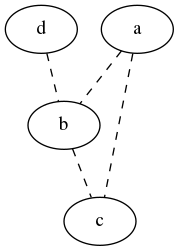
\includegraphics[scale=0.6]{dot/dot_extend_1.png}
     
      \caption{Startgraph}
      \label{fig:algo:extend:1}
   \end{subfigure}&
   \begin{subfigure}[b]{0.32\textwidth}
      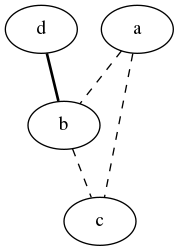
\includegraphics[scale=0.6]{dot/dot_extend_2.png}
     
      \caption{Kante (d,b) wird erfolgreich hinzugefügt}
      \label{fig:algo:extend:2}
    \end{subfigure}&
    \begin{subfigure}[b]{0.32\textwidth}
       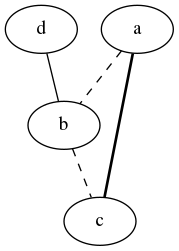
\includegraphics[scale=0.6]{dot/dot_extend_3.png}
    
      \caption{Kante (a,c) erfolgreich wird hinzugefügt}
      \label{fig:algo:extend:3}
    \end{subfigure}
  \end{tabular}
  
    \begin{tabular}[c]{ccc}
    \begin{subfigure}[b]{0.32\textwidth}
     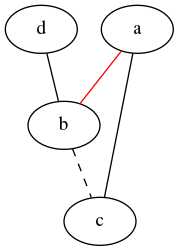
\includegraphics[scale=0.6]{dot/dot_extend_4.png}
    
      \caption{Kante (a,b) kann nicht hinzugefügt werden}
      \label{fig:algo:extend:4}
   \end{subfigure}&
   \begin{subfigure}[b]{0.32\textwidth}
    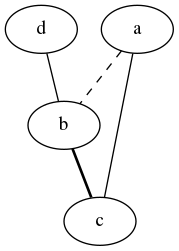
\includegraphics[scale=0.6]{dot/dot_extend_5.png}
      \caption{Kante (b,c) kann nicht hinzugefügt werden}
      \label{fig:algo:extend:5}
    \end{subfigure}&
    \begin{subfigure}[b]{0.32\textwidth}
     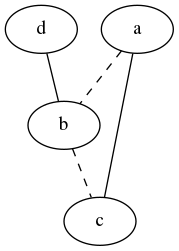
\includegraphics[scale=0.6]{dot/dot_extend_6.png}
    
      \caption{Resultierender Graph}
      \label{fig:algo:extend:6}
    \end{subfigure}
  \end{tabular}
  \caption{Beispielweiser Ablauf des Extends-Algorithmus}\label{fig:algo:extend}
\end{figure}

\subsection{GRASP-Ansatz}
Nach dem experimentellen Untersuchen der Forward und Backward-Ansätze wurden deren Stärken und Schwächen deutlich. So entstand auch die Idee diese beiden Ansätze zu kombinieren. Nach dem Planen und der Umsetzung einer solchen kombinierten Heuristik, hat die Recherche ergeben, dass eine sehr ähnliche Art von Algorithmen bereits beschrieben wurde und unter dem dem Namen GRASP (Greedy Randomized Adaptive Search Procedure) \cite{Feo95,Bastos2014} bekannt ist. Es ist eine iterative Vorgehensweise, wobei jede Iteration aus zwei Phasen besteht: 
\begin{itemize}
\item \textbf{Konstruktions-Phase.} Es wird mit einem leeren Graphen angefangen und es werden iterativ  Knoten/Kanten nach einem bestimmten Kriterium hinzugefügt.
\item \textbf{Lokale Suche.} Da die Lösung, die in der Konstruktions-Phase generiert wurde, meistens nicht optimal ist, auch nicht in der einfachen Nachbarschaft. Deswegen wird in der lokalen Suche versucht die Lösung zu verbessern, indem man nach und nach die derzeitige Lösung durch eine bessere Lösung in der Nachbarschaft ersetzt.
\end{itemize}
Dieser GRASP Ansatz wurde bereits erfolgreich für das Biclustering-Problem verwendet \cite{De12}.

Unsere Ansätze unterscheidet sich darin von den GRASP-Algorithmen, dass wir nicht in jeder Iteration einen neuen Graphen konstruieren, sondern auf dem bereits konstruierten Graphen weiter arbeiten. 

\subsubsection{Grow-Reduce}
Der Grow-Reduce-Ansatz sieht wie folgt aus: Begonnen wird mit einem Graphen, der die selben Knoten wie der Eingabegraph hat aber keine Kanten. Dann wird in jeder Iteration ein Knoten und seine Nachbarschaft hinzugefügt und durch lokale Suche werden alle neu entstandenen verbotenen Teilgraphen wieder entfernt. Dies ist im Algorithmus \ref{algo:growReduce} zu sehen.  Die Grow-Phase ist mit der Konstruktion-Phase des GRASP-Ansatzes vergleichbar und die Reduce-Phase mit der lokalen Suche.

\textbf{Sortierung:}\\
Sowohl in  Grow-Reduce als auch in Explorerd-Grow-Reduce Algo werden die Knoten mittels der Funktion \func{order} sortiert und dann eine nach der anderen abgearbeitet. Nun kann man die Knoten nach unterschiedlichen Kriterien sortieren.
Es wurden 3 Sortierfunktionen verwendet:
\begin{itemize}
\item \textbf{Random}: Zufällig. Das ist die einfachste und offensichtliches Sortierfunktion. Wenn keine Informationen über die Struktur der Daten vorhanden sind, dann ist das zufällige Abarbeiten der Knoten naheliegend.
\item  \textbf{Neighbors}: Anzahl der Nachbarn. Die Knoten werden nach der Anzahl der Nachbarn im Eingabegraphen sortiert.
\item  \textbf{Hits}: Anzahl von verbotenen Teilgraphen. Die Knoten werden danach sortiert, wie oft der Knoten in einem verbotenen Teilgraphen vorkam.
\end{itemize}
Bei den letzten beiden Sortiergmöglichkeiten gibt es sowohl die aufsteigende als auch die absteigende Variante. \\

\textbf{Lokale Suche:}
Bei der lokalen Suche oder der Reduce-Phase wird ein verbotener Teilgraph gesucht und eine zufällige Kante in diesem geändert. Dabei wird ein Kovergenzkriterium verwendet, welches besagt, dass nach der Änderung der Anzahl der verbotenen Teilgraphen kleiner werden soll. Wenn dieses nicht erfüllt wird, dann wird die Änderung wieder rückgängig gemacht.\\



\textbf{Zeitlimit:}
Da bei der Entwicklung festgestellt wurde, dass eine Iteration duch alle Knoten zeitlich sehr umfangreich ist, wurde die Tatsache ausgenutzt, dass in jeder Iteration wir einen validen Graphen haben. Das bedeutet, dass man nach jeder Iteration abbrechen und den Graphen zurückgeben könnte. Dies wäre jedoch suboptimal, deswegen wird der schnelle Extend-Algorithmus vor der Rückgabe der Graphs nochmal auf den Graphen angewandt und dann erst wird der Graph zurückgegeben.
Die Entscheidung, nach welcher Iteration abzubrechen ist, hängt von dem Zeitlimit ab, wie lange das Programm zu laufen hat.

\begin{algorithm}
  \captionof{algorithm}{GrowReduce}\label{algo:growReduce}
\begin{algorithmic}[1]
\Function{GrowReduceSolve}{$G$, \cursive{F}}
	\State{\vars{graph} $\gets$ $(V(G),\emptyset)$}
	\State{\vars{nodes} $\gets$ \func{order}($V(G)$)}
	\For{\vars{node} $\in$ \vars{nodes}}
		\For{\vars{neighbor} $\in$ $N(\vars{node})$}\Comment{Grow}
			\State{Add edge (\vars{node}, \vars{neighbor}) to \vars{graph}}
		\EndFor
	
			\While{\vars{forbidden} $\gets$ \func{findFS}(\vars{graph}, \cursive{F})}	\Comment{Reduce}
				\State{\vars{edge} $\gets$ \func{randomEdge}(\vars{forbidden})}
				\State{\vars{count} $\gets$ |(\func{findAllFS}(\vars{graph},\cursive{F})|}
				\State{flip \vars{edge} in \vars{graph}}
				\State{countAfter $\gets$ |(\func{findAllFS}(\vars{graph},\cursive{F})|}
				\If{\vars{countAfter} $\geq$ \vars{count}}
					\State{flip \vars{edge} in \vars{graph}}
				\EndIf
			\EndWhile
		
	\EndFor
\Return{\func{solveExtend}(\vars{graph}, \cursive{F})}
\EndFunction
\end{algorithmic}
\end{algorithm}

\subsubsection{Explored-Grow-Reduce}
Der Explored-Grow-Reduce-Ansatz ist dem Grow-Reduce-Ansatz ähnlich, bis auf das, es in der Grow-Phase nur die Kanten zu Knoten hinzufügt, die bereits erforscht sind.

Dieser Unterschied wird in der Abbildung \ref{fig:algo_explored} verdeutlich, wo nur die Grow-Schritte visualisiert wurden, ohne die Reduce-Phase, um die Erklärung zu vereinfachen. In der Abbildung \ref{fig:algo_explored_1} ist der Anfangstatus zu sehen. Die gestrichelten Kanten sind Kanten, die im  Eingabegraphen vorhanden sind, aber noch nicht hinzugefügt worden sind. In der Abbildung \ref{fig:algo_explored_1} wird nun der Knoten $a$ hinzugefügt, weil aber keine anderen Knoten bisher hinzugefügt worden sind, werden auch keine Kanten hinzugefügt.
In Abbildung \ref{fig:algo_explored_2} wird der Knoten $b$ hinzugefügt und weil $a$ auch schon hinzugefügt wurde, wird auch die Kante $(a,b)$ hinzugefügt. Aber weder $(a,c)$ noch $(a,b)$ werden hinzugefügt, weil $c$ noch nicht erforscht wurde.
In Abbildung \ref{fig:algo_explored_3} wird der Knoten $c$ hinzugefügt und somit auch die Kanten $(a,b)$ und $(a,c)$.

Im Grow-Reduce-Ansatz werden im ersten Schritt auch die Kanten zu $b$ und $c$ hinzugefügt werden. Dies wäre im Beispiel vom $P_3$ als verbotenen Teilgraphen aber suboptimal, denn dann wäre der Teilgraph mit den Knoten $a$,$b$ und $c$ ein vom $P_3$ induzierter Teilgraph.
	
	
\begin{figure}
  \centering
  \begin{tabular}[c]{ccc}
    \begin{subfigure}[b]{0.32\textwidth}
      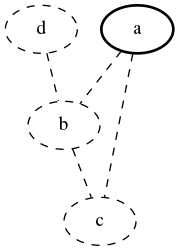
\includegraphics[scale=0.5]{dot/dot_explored_1.png}
     
      \caption{Knoten a wird hinzugefügt}
      \label{fig:algo_explored_1}
   \end{subfigure}&
	 \begin{subfigure}[b]{0.32\textwidth}
	   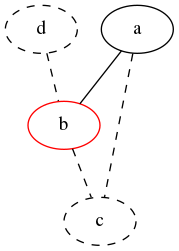
\includegraphics[scale=0.5]{dot/dot_explored_2.png}
	    \caption{Knoten b wird hinzugefügt}
	    \label{fig:algo_explored_2}
	  \end{subfigure}&
    \begin{subfigure}[b]{0.32\textwidth}
      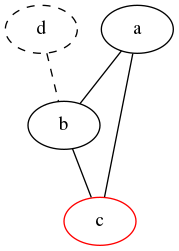
\includegraphics[scale=0.5]{dot/dot_explored_3.png}
	 
	    \caption{Knoten c wird hinzugefügt}
	    \label{fig:algo_explored_3}
    \end{subfigure}
  \end{tabular}
  \caption{Beispielweise Grow-Phase}\label{fig:algo_explored}
\end{figure}

\begin{algorithm}
  \captionof{algorithm}{ExploredGrowReduce}\label{algo:ExploredGrowReduce}
\begin{algorithmic}[1]
\Function{ExploredGrowReduceSolve}{$G$, \cursive{F}}
	\State{\vars{graph} $\gets$ $(V(\vars{G}),\emptyset)$}
	\State{\vars{nodes} $\gets$ \func{order}($V(G)$)}
	\State{\vars{explored} $\gets \emptyset$}
	\For{\vars{node} $\in$ \vars{nodes}}
		\For{\vars{neighbor} $\in$ N(\vars{node})}\Comment{Grow Phase}
			\If{\vars{neighbor} $\in$ \vars{explored}}
				\State{Add Edge (\vars{node}, \vars{neighbor}) to \vars{graph}}
			\EndIf
		\EndFor \\
		\Comment{Reduce Phase}
			\While{\vars{forbidden} $\gets$ \func{findFS}(\vars{graph}, \cursive{F})}
				\State{\vars{edge} $\gets$ \func{randomEdge}((\vars{forbidden})}
				\State{\vars{count} $\gets$ |(\func{findAllFS}(\vars{graph},\cursive{F})|}
				\State{flip \vars{edge} in \vars{graph}}
				\State{countAfter $\gets$ |(\func{findAllFS}(\vars{graph},\cursive{F})|}
				\If{\vars{countAfter} $\geq$ \vars{count}}
					\State{flip \vars{edge} in \vars{graph}}
				\EndIf
			\EndWhile
	\EndFor
\Return{\func{solveExtend}(\vars{graph}, \cursive{F})}
\EndFunction
\end{algorithmic}
\end{algorithm}

\subsection{Ganzzahlige lineare Optimierung}
Bei der linearen Optimierung wird eine lineare Zielfunktion minimiert bzw. maximiert, wobei sie durch lineare Gleichungen und Ungleichungen beschränkt ist.

Wir nutzen binäre Variablen $e_{uv}$, wobei $u,v \in V$ sind und $u < v$ gilt.
Dabei ist $e_{uv} = 1$ genau dann wenn, die kante ${u,v}$ ein Teil des Lösungsgraphen ist.

Wir minimieren \[\sum_{u,v \in V} 
\begin{cases} 
      e_{u,v} & \{u,v\} \in E \\
      -e_{u,v} & \{u,v\} \notin E
   \end{cases}\]
Dies ist die Zielfunktion \vars{objective} im Algorithmus \ref{algo:bip}.

Da alle möglichen Bedingungen hinzuzufügen, welche alle verbotenen Teilgraphen ausschließen würden, viel zum umfangreich wäre, werden die Bedingungen iterativ dort hinzugefügt, wo es einen verbotenen Teilgraphen gibt. Dann wird das Problem mittels Binary-Linear-Programming gelöst und die Änderungen auf den Graphen übertragen. Dann wird wieder nach allen verbotenen Teilgraphen gesucht. Dies wird solange wiederholt bis es keine mehr gibt. Damit ist die minimale Anzahl von Änderungen gefunden. 
\begin{algorithm}
  \captionof{algorithm}{F-Free BIP}
  \label{algo:bip}
\begin{algorithmic}[1]
\Function{solveBIP}{$G$, \cursive{F}}
    \State{\vars{constraints} $\gets$ $\emptyset$}
    \While{not \func{isValid}($G$, \cursive{F})}
	    \For{$f$ $\in$ \func{findAllFS}($G$,  \cursive{F})}\label{algo:bip:findFS}
			\State{\vars{c} $\gets$ 0}
			\For{each $\{u,v\}$ mit $u \in Bild(f) \land v \in Bild(f) \land u \neq v $}
				\If{$\{u,v\}$ $\in$ $E(G)$} 
					\State{\vars{c} += 1 - $e_{uv}$} 
				\Else 
					\State{\vars{c} += $e_{uv}$} 
				\EndIf
			\EndFor
			\State{\vars{constraints} $\gets$ \vars{constraints} $\cup$ \{ \vars{c} \}}
		\EndFor
		\State{\vars{variables} $\gets$ \func{BIPSolve}(\vars{constraints}, \vars{objective})}\label{algo:bip:solve}
		\For{$e_{u,v}$ $\in$ \vars{variables}} \Comment{Apply solution to the graph.}\label{algo:bip:apply}
		  \If{$e_{u,v} = 1$}
		    \State{Set edge $(u,v)$ in $G$}
		  \Else
		    \State{Remove edge $(u,v)$ in $G$}
		  \EndIf
		\EndFor
	\EndWhile
\Return{$G$}
\EndFunction
\end{algorithmic}
\end{algorithm}


\newpage 
\section{Aufbau der Experimente}

\label{sec:tests}
\subsection{Datensätze}
Da verschiedene Mengen von verbotenen Teilgraphen monotonen Grapheneigenschaften zugeordnet werden können und jeder Datensatz von Graphen und jede Methode zufällige Graphen zu erzeugen, charakteristische Eigenschaften hat, ist es notwendig verschiedene Datensätze zu verwenden und verschiedene Methoden zur Erzeugung von zufälligen Graphen.
Insgesamt wurde 5 verschiedene Methoden zur Erzeugung von zufälligen Graphen verwendet und 3 Datensätze.
Wir brachten zuerst die zufälligen Graphen und dann einige Graphen basierend auf realen Modellen.


\subsubsection{Barabási–Albert}
Für den Datensatz \vars{barabasi\_albert} wurde das Barabási–Albert Modell verwendet, welches ein zufälliges skalenfreies Netz erzeugt\cite{Albert02}.
Skalenfrei bedeutet hier, dass die Knotengrad einer Potenzverteilung folgt. Es gibt also viel mehr Knoten, die einen geringeren Grad haben als Knoten mit einem hohen Anzahl von Nachbarn. 

Es wurden 56 Graphen generiert mit Knotenanzahl in $\{10,20,30, \ldots, 140\}$, mit dem Parameter $m \in \{1,3,5,7\}$, welcher die Anzahl der der Kanten definiert, die zu bereits bestehenden Knoten erstellt werden.
\subsubsection{Erdős-Rényi}
Für den Datensatz \vars{ER} wurde das Erdős-Rényi Modell verwendet\cite{Gilbert59,Batagelj05} wo jede Kante eine fixe Wahrscheinlichkeit hat zu existieren oder nicht zu existieren.

Es wurden dabei 54 Graphen generiert, mit einer Knotenanzahl $n \in \{10,20, \ldots ,90\}$ und den folgenden Wahrscheinlichkeiten: $\frac{1}{10}$, $\frac{2}{10}$, $\frac{5}{20}$, $\frac{4}{10}$, $\frac{5}{10}$, $\frac{8}{10}$.


\subsubsection{Duplication-Divergence}
Für den Datensatz \vars{duplication\_divergence} wurde das Duplication Divergence Modell verwendet\cite{Ispolatov05}, welches Interaktionsnetzwerke zwischen Proteinen modelliert. Ein Beispiel ist in Abbildung \ref{fig:duplication-divergence} zu sehen.

Dabei gibt es in jeder Iteration bei der Erstellung eines solchen zufälligen Graphen zwei Phasen. Die erste ist die Duplikations-Phase, wo ein zufälliger Knoten $u$ genommen und dupliziert wird zu $v$. Dann beginnt die Divergence-Phase, wo zu jedem Nachbarn von $u$ mit gewissen Wahrscheinlichkeit $p$ eine Kante zu $v$ hinzugefügt wird. Falls keine Kanten hinzugefügt wurde, dann wird $v$ wieder gelöscht. Dies wird $n$-mal wiederholt 

Es wurden mit diesem Modell 54 Graphen generiert mit $n \in \{10,20, \ldots,90\}$. Für die Wahrscheinlichkeiten $p$ wurden folgende Werte verwendet $\frac{1}{10}$, $\frac{2}{10}$, $\frac{5}{20}$, $\frac{4}{10}$, $\frac{5}{10}$, $\frac{8}{10}$.
\begin{figure}
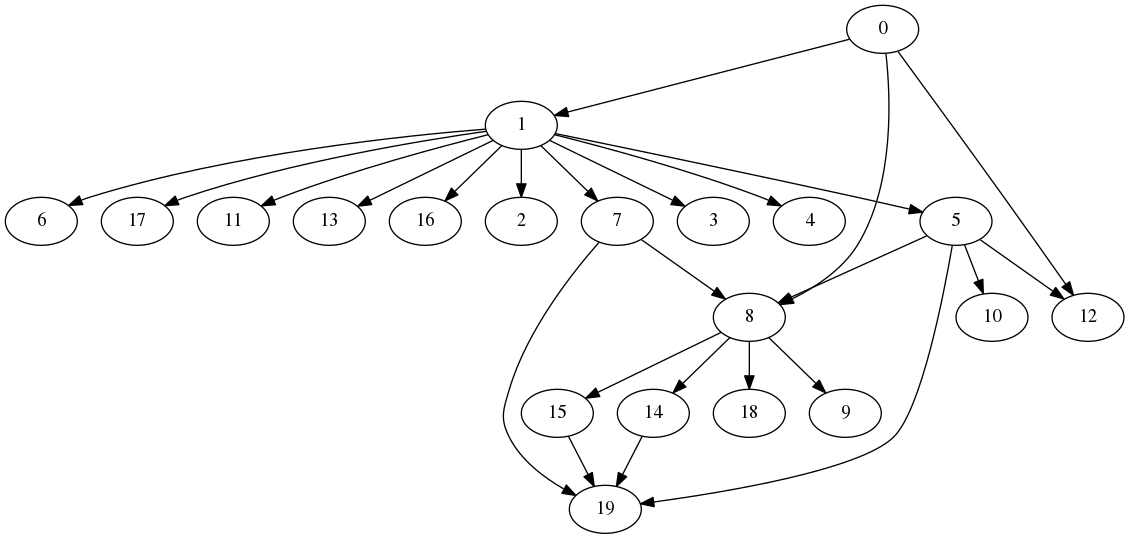
\includegraphics[scale=0.35]{dot/dot_dupdivergence.png}
\caption{Ein beispielhafter Duplication-Divergence Graph mit $n$ = 20 und $p$ = 0,4}
\label{fig:duplication-divergence}
\end{figure}

\subsubsection{Newman-Watts-Strogatz}
Für den Datensatz \vars{newman\_watts\_strogatz} wurde das Newman-Watts-Strogatz Modell verwendet\cite{Newman99}, welches Kleine-Welt-Graphen erzeugt mit einer geringen durchschnittlichen Knotendistanz und einem hohen Clusterkoeffizienten.

Dabei wird zuerst ein Kreis von $n$ Knoten erstellt. Dann wird jeder Knoten mit $k$ von seinen nächsten Nachbarn verbunden (oder mit $k-1$, wenn $k$ ungerade ist).
Dann werden Abkürzungen erzeugt, indem man für jede Kante $(u,v)$ in dem zugrunde liegenden $n$-Kreis mit den $k$ nächsten Nachbarn, folgendes tut: Füge mit der der Wahrscheinlichkeit $p$ eine neue Kante $(u,w)$ ein, wobei $w$ ein zufällig gewählter Knoten ist.

Es wurden mit diesem Model 144 Graphen generiert mit einer Knotenanzahl $n \in \{10,20, \ldots,90\}$  , $k \in \{2,4,6,8\}$ und der Wahrscheinlichkeit $p \in \{\frac{2}{10},\frac{4}{10},\frac{6}{10},\frac{8}{10}\}$.
\subsubsection{Powerlaw-Baum}
Für den Datensatz \vars{powerlaw}, wurde ein Modell verwendet, dass einen Baum erzeugt, dessen Knotengrad einer Potenzverteilung folgt \cite{Aiello01}. Ein Beispiel ist in Abbildung \ref{fig:powerlaw-tree} zu sehen.
Es wurden mit diesem Model 30 Graphen generiert mit einer Knotenanzahl zwischen $n \in \{10,15,20, \ldots,155\}$.
\begin{figure}
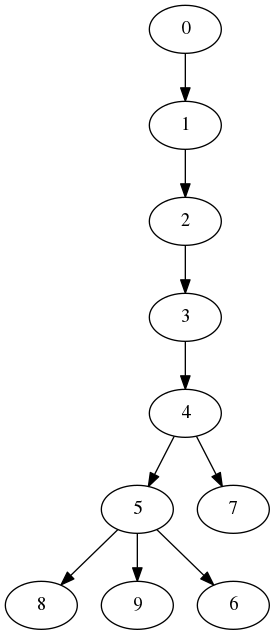
\includegraphics[scale=0.35]{dot/dot_powerlaw.png}
\caption{Ein Powerlaw-Baum mit $n$ = 10}
\label{fig:powerlaw-tree}
\end{figure}

\subsubsection{Netzwerke}
Für den Datensatz \vars{UCINetworkDataRepository} wurden 9 reale Graphen verwendet, bereitgestellt von der University of California.
\begin{itemize}
\item Der Graph \vars{karate} ist ein soziales Netzwerk von Freundschaften zwischen 34 Mitgliedern eines Karate-Clubs in einer US-Universität in 1970 \cite{Zachary77}.
\item Der Graph \vars{polbooks} ist ein Netzwerk von Bücher über die aktuelle US Politik, die von dem Onlinehänder Amazon.com verkauft wurdem. Kanten repräsentieren häufiges Kaufen von den beiden Büchern von dem selben Käufer \cite{polbooks}.
\item Der Graph \vars{football} ist ein Netzwerk von amerikanischen Footballspielen im Herbst 2000 \cite{Girvan02}.
\item Der Graph \vars{power} ist ein Netzwerk, dass die Topologie des "Western States Power Grid" in der Vereinigten Staaten wiederspieglt  \cite{Watts98}.
\item Der Graph \vars{adjnoun} ist ein Netzwerk von häufigen Adjektiven und Nomen in dem Roman "David Copperfield" von Charles Dickens \cite{Newman06}.
\item Der Graph \vars{lesmiserables} ist ein Netwerke von Figuren, die in dem  Roman "Les Misérables" von Victor Hugo, zur gleichen Zeit auftreten \cite{Knuth93}. 
\item Der Graph \vars{celegansneural} welches das neurale Netzwerk von Caenorhabditis elegans \cite{Watts98}. Es ist ein Fadenwurm, welcher gerne als Modellorganismus studiert wird. Jeder erwachsene C. elegans hat genau 302 Nervenzellen.
\item Der Graph \vars{dolphins} ist ein soziales Netzwerk von 62 Dolphinen die in einer Gemeinschaft in der Nähe von Neuseeland leben \cite{Lusseau03}. 
\item Der Graph \vars{polblogs} ist ein Netzwerk von Hyperlinks zwischen Webblogs in 2005, die sich mit auf US Politik beschäftigten \cite{Adamic05}.
\end{itemize}



\subsubsection{Squenzähnlichkeit von Proteinen}
Der Datensatz  \vars{bio1} umfasst 147 Graphen und der \vars{bio2} umfasst 350 Graphen. Beide sind Graphen die Squenzähnlichkeit von Proteinen modellieren \cite{Rahmann07,Bocker08}.

\subsection{Details der Experimente}
Um nachvollziehbare, fehlerarme und detaillierte Resultate der Experimente zu erhalten, wurde eine Umgebung implementiert, die automatisch die Experimente laufen lässt, die Daten sammelt und diese auswertet.

Dafür werden Experimente in einer Konfigurationsdatei definiert, indem folgende Informationen dort aufgelistet werden: Datensätze, \cursive{F},  Algorithmen und die maximale Laufzeit. Diese Information wird genutzt, um dann die Experimente automatisch laufen zu lassen. Dabei wird bei jedem Experiment unter anderem die Laufzeit, der maximaler Speicherverbrauch, die Anzahl der Änderungen, der resultierende Graph und Informationen, um das Verhalten des Algorithmus nach zu vollziehen, gesammelt.

Um die Qualität der Lösung eines heuristischen Ansatzes bewerten zu können, ist es notwendig die optimale Lösung zu wissen. Es gibt verschiedene Ansätze wie das Problem zu lösen sein, wir haben uns jedoch für die binäre lineare Optimierung entschieden. Der BIP-Algorithmus versucht eine optimale Lösung zu finden. Dies kann jedoch sehr lange dauern, da das Problem NP-vollständig ist. 
In der Tabelle \ref{tab:size_solved_bio2} sehen wir, dass für einige verbotene Teilgraphen wir für alle Instanzen eine optimale Lösung berechnen konnten, aber es gibt schwierige verbotene Teilgraphen wie ($P_5$, triangle) wo wir für die meisten Instanzen keine optimale Lösung berechnen konnten.
\begin{center}
\captionof{table}{Nicht gelöste Instanzen für den Datensatz \vars{bio2}}
\label{tab:size_solved_bio2}
\begin{tabular}{ccc}
\hline 
Verbotener Teilgraph & Anzahl & Prozent \\ 
\hline
$2 P_3$ & 0 & 0\% \\ 
$C_4$ & 0 & 0\% \\ 
claw & 0 & 0\% \\ 
paw & 4 & 1\% \\ 
triangle & 11 & 3\% \\ 
splitcluster & 26 & 7\% \\ 
($P_4,C_4)$ & 37 & 10\% \\ 
(x172, triangle) & 129 & 36\% \\ 
($P_5$, triangle)& 309 & 86\% \\ 
\hline
\end{tabular} 
\end{center}

Des weiteren wurden für jeden Graphen in den Datensätzen folgende Variablen bestimmt, die Anzahl der Knoten, die Anzahl der Kanten, die minimale / maximale / durchschnittliche Anzahl von Nachbarn, der minimale / maximale / durchschnittliche Clustering-Koeffzient, Degeneracy und Dichte.

Die Resultate der Experimente kann man mittels einer webbasierten Benutzeroberfläche interaktiv untersuchen. So ist es beispielsweise möglich  die Auswirkung der Dichte der Graphen auf die Laufzeit in einem Linendiagramm darstellen zu lassen. Oder die Auswirkung der der durchschnittlichen Dichte auf die normierte Lösungsgröße. Diese Benutzeroberfläche für Resultate von den Experimenten ist unter  \url{http://metaxy.github.io/f-free-browser-data/} zu finden.

\subsection{Implementierungsdetails}

\label{sec:implementation}
\subsubsection{Allgemein}
Die Algorithmen wurden in der Sprache C++14 implementiert. Für die Repräsentation der Graphen wurde eine einfache Adjazenzmatrix verwendet. Der Code ist unter \cite{Code} zu findenFür das Binary-Integer-Programming wurde Gurobi 6.5 verwendet \cite{gurobi}.

Für das Finden von verboten Teilgraphen haben wir Bibliotheken verwendet, die das Graphen-Subgraph Isomorphismus Problem implementieren.
Da das Finden von induzierten Teilgraphen der zeitaufwendigste Teil der Algorithmen ist, ist hier die Wahl von dem richtigen Ansatz sehr wichtig. Hier werden drei Ansätze bezüglich ihrer Geschwindigkeit verglichen, wobei der $P_3$ der verbotene Teilgraph ist. 

\begin{itemize}
\item Der Ansatz erste ist VFLib. Es ist ein Bibliothek, die mehrere VF2-Algorithmen \cite{Cordella04} jeweils für das Graphen-Isomorphismus-Problem, Graphen-Subgraph-Isomorphismus-Problem und das Graphen-Monomorphimus Problem-implementiert und zählt zu den schnellsten Implementationen.

\item Der zweite Ansatz nutzt die Boost-Implementation von VF2, welches VFLib auch implementiert.

\item Im dritten Ansatz wird die Suche nach dem $P_3$ selbst möglichst effizient implementiert. 
\end{itemize}

Hierbei vergleichen wir nicht die verschiedenen Algorithmen für das Graph-Subgraph Isomorphismus Problem, weil VFLib und Boost den selben grundlegenden Ansatz verwenden und die eigene Implentieren gar kein Graph-Subgraph Isomorphismus Algorithmus ist. Vielmehr geht es darum, herausfinden wie groß ungefähr der Overhead ist und ob eine Optimierung lohnenswert wäre.

Die drei unteschiedlichen Anwendungsfälle sind:
\begin{itemize}
 \item \textbf{Alle Finden}: Finde und gebe alle verbotenen Teilgraphen zurück
 \item \textbf{Alle Zählen}: Zählen wie viele verbotene Teilgraphen der Graph hat
 \item \textbf{Einen zurückgeben}: Finde einen verbotenen Teilgraphen und gebe ihn zurück.
\end{itemize}

In Tabelle \ref{tab:benchmark_isomorph} werden die Resultate anzeigt, dabei gibt die Zeit an, wie lange es gebraucht hat die Aufgabe auf allen 147 Graphen von dem Datensatz \vars{bio1} auszuführen. In der Zeit ist die Zeit für das Einlesen der Graphen nicht mit einbegriffen. Die Werte unter der Zeit, sind Angaben, wie viel mal langsamer der Ansatz als der schnellste Ansatz ist.
\begin{table}

\centering

\begin{tabular}{c ccc}
\hline 
Verfahren & Alle finden & Alle zählen & Einen zurückgeben \\ 
\hline 
VFLib & 1,73s (2,4x) & 0,87s (22x) & 0,0124s (77x) \\ 
Boost & 3,04s (4,2x) & 1,68s (42x) & 0,00102s (6,4x) \\ 
Naive $P_3$-Suche & 0,73s & 0,04s & 0,00016s \\ 
\hline 
\end{tabular} 
\caption{Laufzeitvergleich von VFLib, Boost und Naive P3-Suche}
\label{tab:benchmark_isomorph}
\end{table}
Zu sehen ist, dass die "Naive $P_3$-Suche" viel schneller ist, aber es ist auch zu beachten, dass VFLib und Boost allgemeine Ansätze sind, während die naive $P_3$-Suche nur für den Graphen $P_3$ funktioniert. 

Zu beobachten ist auch, dass VFLib bei dem \glqq Alle finden\grqq \, und \glqq Alle zählen\grqq \, deutlich schneller ist, aber beim \glqq Einen zurückgeben\grqq \, weitaus langsamer ist. Dies hat mit dem Benchmark selbst zu tun. Weil dort die Algorithmen sehr schnell sind, wurde es 100-mal auf jedem Graphen ausgeführt. Dann wurde die Zeit durch 100 dividiert. 
An sich ist es auch kein Problem, aber der Unterschied liegt in der Tatsache, dass die Datenstruktur von VFLib unveränderlich ist und wir bei jedem Aufruf einen neuen Graphen für VFLib erstellen, während bei Boost wir den Graphen nicht immer wieder neu erstellen müssen. Auch wenn man den Benchmark anders gestalten könnte, wurde er absichtlich so gestaltet, weil es in den Heuristiken eine reale Anwendung ist: Oft wird wiederholt eine Änderung gemacht und dann nach einem verbotenen Teilgraphen gesucht. Hier wäre der Boost-Ansatz also weitaus besser, weil man nach einer jeder Änderung nicht einen neuen Graphen konstruieren müsste.

Die Schlussfolgerung von diesem Benchmark ist, dass die VFLib und Boost Algorithmen schnell genug sind und höchstens eine Optimierung von \glqq   Alle zählen\grqq \, eine vielversprechende Option wäre.

So auch wurde bei der Implementierung der Algorithmen sowohl VFLib als auch Boost verwendet. Wenn es darum ging immer wieder einen verbotenen Graphen zurückzugeben, dann wurde Boost verwendet und es darum ging vor allem häufig die Anzahl der verbotenen Teilgraphen zählen oder alle verbotenen Teilgraphen zu zählen, dann wurde VFLib verwendet.
\newpage
\section{Auswertung}
\label{sec:results}

In diesem Abschnitt werden wir die Auswertung der Tests vornehmen, indem wir zuerst die Algorithmen betrachten, welche einige Instanzen nicht lösen konnten. Dann werden wir die Lösungsqualität und den Zeitaufwand der Heuristiken untersuchen. Zum Schluss wird die Wahl der Sortierfunktion für die Grow-Reduce-Ansätze untersucht. Die Experimente wurden auf einem Intel 3Ghz Dual-Core (BX80637G2030) mit 8 GB RAM ausgeführt.
Die Resultate der Tests sind unter \cite{Benchmark} zu finden. Auch können sie interaktiv unter folgender URL untersucht werden: \url{http://metaxy.github.io/f-free-browser-data/}.

\subsection{Nicht gelöste Instanzen}
Die beiden Backward-Ansätze RandomFlip und RandomFlipUnchanged haben im Gegensatz zu den anderen Algorithmen viele Instanzen, die sie in der vorgegebenen Zeit nicht lösen konnten. In der Tabelle \ref{tab:benchmark_notsolved} ist die Anzahl der nicht gelöste Instanzen auf den \vars{bio2} Daten bei einer maximalen Laufzeit von 10s zu sehen. Zu beachten ist, dass der Datensatz \vars{bio2} nur 350 Graphen hat. 

Die Ursache für die hohe Anzahl der ungelösten Instanzen bei RandomFlip liegt darin, dass bei RandomFlip der Algorithmus nicht nach kurzer Zeit terminieren muss. Es wird jedes Mal eine zufällige Kante/Nicht-Kante aus dem ersten gefundenen verbotenen Teilgraphen genommen.
So kann es sein, dass wenn die minimale Anzahl der Änderungen am Graphen, um ihn \cursive{F}-frei zu machen, sehr hoch ist. Dann passiert es, dass der Algorithmus lange braucht um überhaupt eine Lösung zu finden. So ist in der Abbildung \ref{fig:not_solved} zu sehen, dass mit größerer Knotenanzahl immer mehr Instanzen von RandomFlip nicht gelöst werden.

\begin{figure}
    \centering
    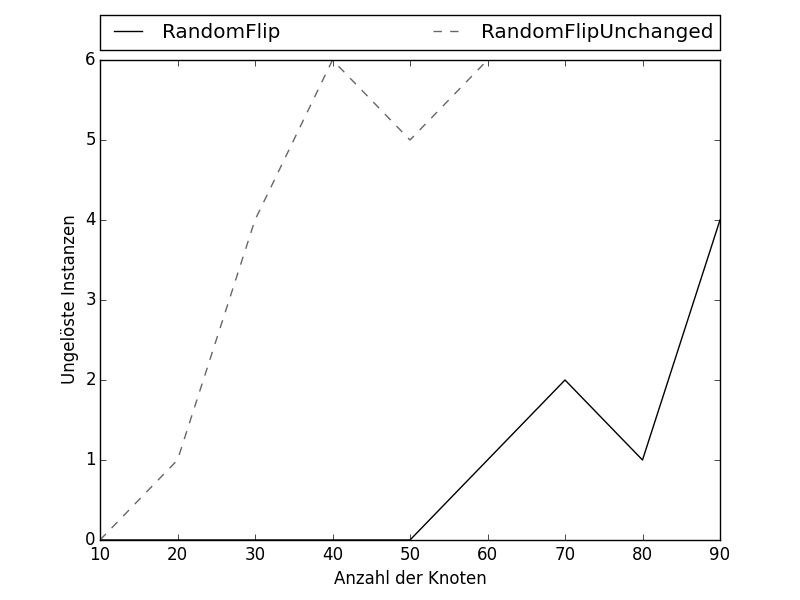
\includegraphics[scale=0.4]{plots/not_solved.png}
    \caption{Anzahl der nicht gelösten Instanzen auf dem \vars{duplication\_divergence} Datensatz für Splitcluster}
    \label{fig:not_solved}
\end{figure}

\begin{table}
\centering
\begin{tabular}{c cc}
\cursive{F} &  RandomFlip & RandomFlipUnchanged  \\ 
\hline 
Splitcluster & 253 & 17 \\
Cluster & 293 & 54 \\
Co-Graph & 251 & 12 \\
x172 triangle & 320 & 31 \\
Quasi-Threshold & 250 & 15 \\
Split & 254 & 10  \\
$K_{14}$ Paw & 266 & 31\\
\end{tabular} 
\caption{Anzahl nicht gelöster Instanzen auf dem \vars{bio2} Datensatz}
\label{tab:benchmark_notsolved}
\end{table}


So ist RandomFlipUnchanged deutlich besser, schafft es bei einer größeren Knotenanzahl nicht alle Instanzen zu lösen.
Die Idee, dass man eine einmal geänderte Kante mit einer geringer Wahrscheinlichkeit wieder ändert, hat also den RandomFlip-Algorithmus verbessert. Damit sind die Algorithmen RandomFlip und RandomFlipUnchanged sehr begrenzt nützlich und zwar nur für kleine Graphen. 

\subsection{Lösungsqualität}
In der Abbildung \ref{fig:qual} sind die durchschnittlichen normierten Lösungsgrößen der Algorithmen auf dem \vars{bio2}-Datensatz dargestellt. RandomFlip wurde nicht einbezogen, weil es so viele ungelöste Instanzen hat. Dabei wurden ungelöste Instanzen mit der normierten Lösungsgröße von $0,5$ eingerechnet.
Der Extend-Algorithmus kann bei kleinen Graphen nicht mal mit dem RandomFlipUnchanged-Algorithmus mithalten, außer bei den Split-Graphen. 
Wenn man Abbildung \ref{fig:qual_grow} mit \ref{fig:qual_explored} vergleicht, ist zu sehen, dass der ExploredGrowReduce-Ansatz dem GrowReduce-Ansatz bezüglich der Lösungsgröße überlegen ist. Alles in allem ist der ExploredGrowReduce-Algorithmus bezüglich der Lösungsqualität der Beste.

\begin{figure}
  \centering
  \begin{tabular}[c]{cc}
    \begin{subfigure}[b]{0.5\textwidth}
       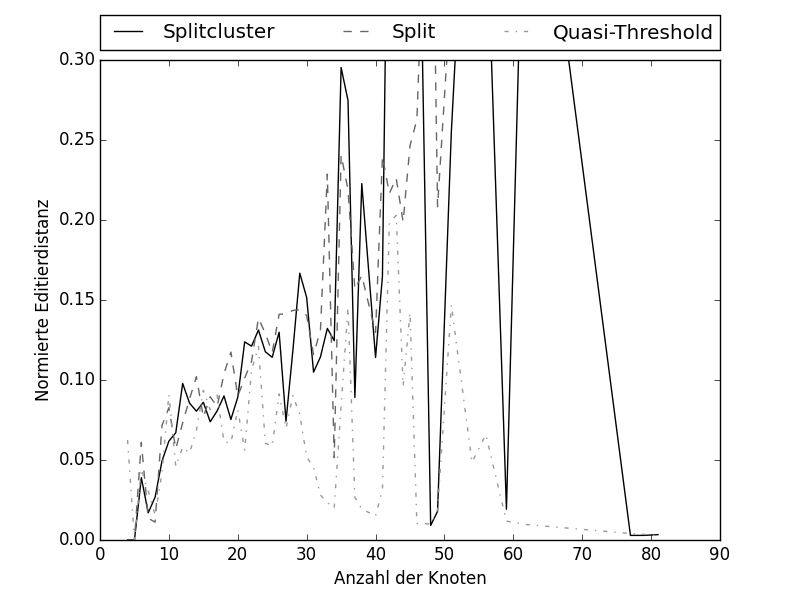
\includegraphics[scale=0.35]{plots/quality_random.png}
       \caption{RandomFlipUnchanged}
       \label{fig:qual_random}
       
    \end{subfigure}&
    \begin{subfigure}[b]{0.5\textwidth}
         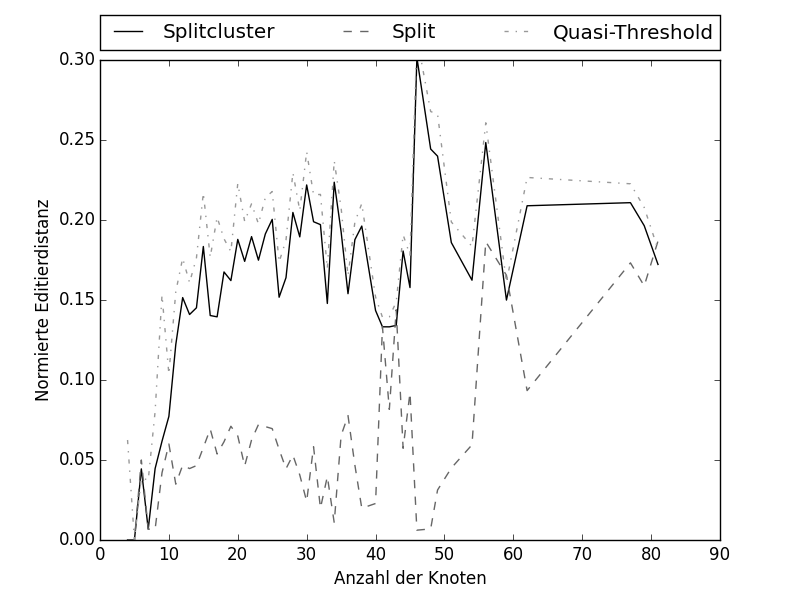
\includegraphics[scale=0.35]{plots/quality_extend.png}
         \caption{Extend}
         \label{fig:qual_extend}
       
    \end{subfigure}
  \end{tabular}
  \begin{tabular}[c]{cc}
    \begin{subfigure}[b]{0.5\textwidth}
       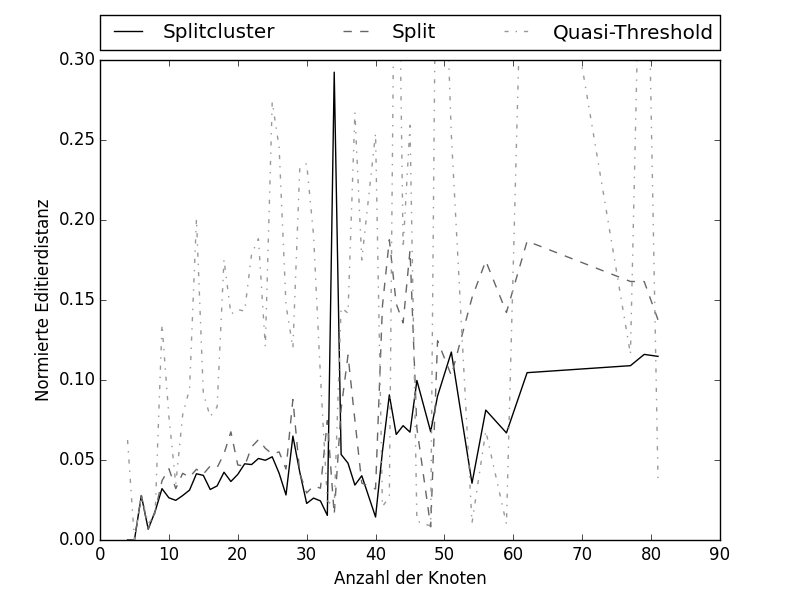
\includegraphics[scale=0.35]{plots/quality_grow_reduce.png}
        \caption{GrowReduce}
       \label{fig:qual_grow}
      
    \end{subfigure}&
    \begin{subfigure}[b]{0.5\textwidth}
        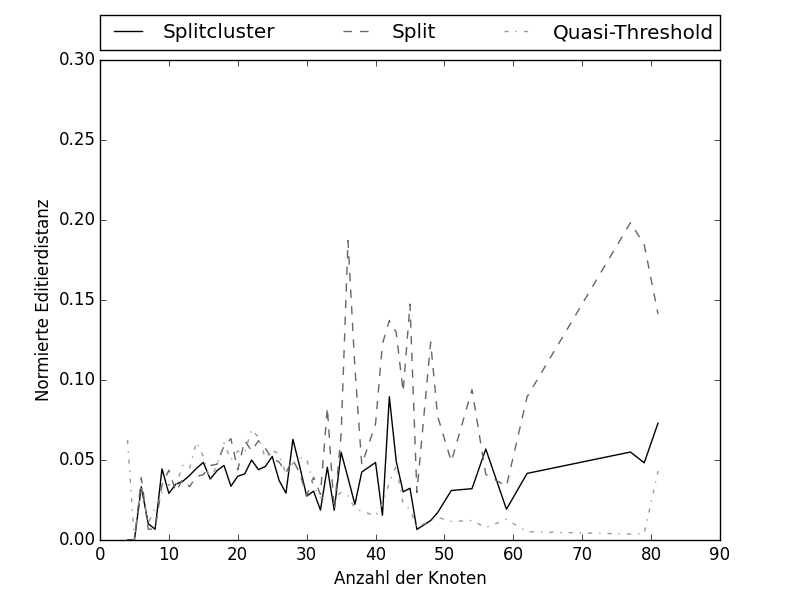
\includegraphics[scale=0.35]{plots/quality_explored_grow.png}
         \caption{ExploredGrowReduce}
         \label{fig:qual_explored}
      
    \end{subfigure}
  \end{tabular}
    \caption{Durchschnittlich normierte Lösungsgröße der Algorithmen auf dem \vars{bio2}-Datensatz}

  \label{fig:qual}
\end{figure}



\subsection{Laufzeit}

In der Abbildung \ref{fig:time} sind zwei Lininiendiagramme, welche die Laufzeit von Extend, GrowReduce und ExploredGrowReduce darstellen. Zu sehen ist, dass sowohl mit der Kantenanzahl, als auch mit der Knotenanzahl die Laufzeit wächst. Dabei ist aber zu beachten, dass sowohl GrowReduce als auch ExploredGrowReduce ein Abbruchkriterium haben. Das heißt, dass wenn sie es nicht schaffen durch alle Knoten zu iterieren, dass sie vorzeitig abbrechen und dann noch den Extend-Algorithmus laufen lassen und dann das Ergebnis zurückgeben. In diesem Experiment war das Zeitlimit 10 Sekunden.

Zu sehen ist auch, dass die Kantenanzahl einen größeren Effekt auf die Laufzeit hat als die Knotenanzahl. Auch ist der Extend-Algorithmus wesentlich schneller als die Grow-Reduce-Ansätze.
\begin{figure}
  \centering
  \begin{tabular}[c]{cc}
    \begin{subfigure}[b]{0.5\textwidth}
        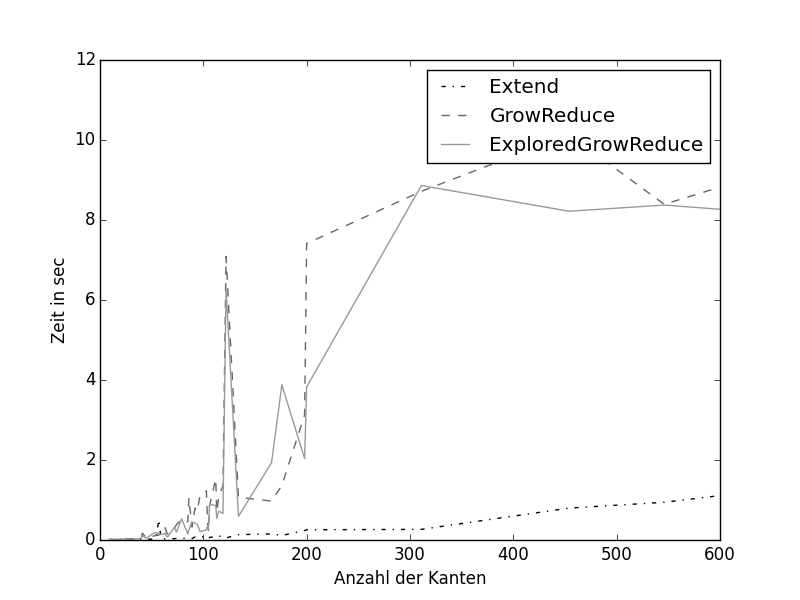
\includegraphics[scale=0.37]{plots/time_edge.png}
       \caption{Kantenanzahl-Zeit-Diagramm}
    \end{subfigure}&
    \begin{subfigure}[b]{0.5\textwidth}
        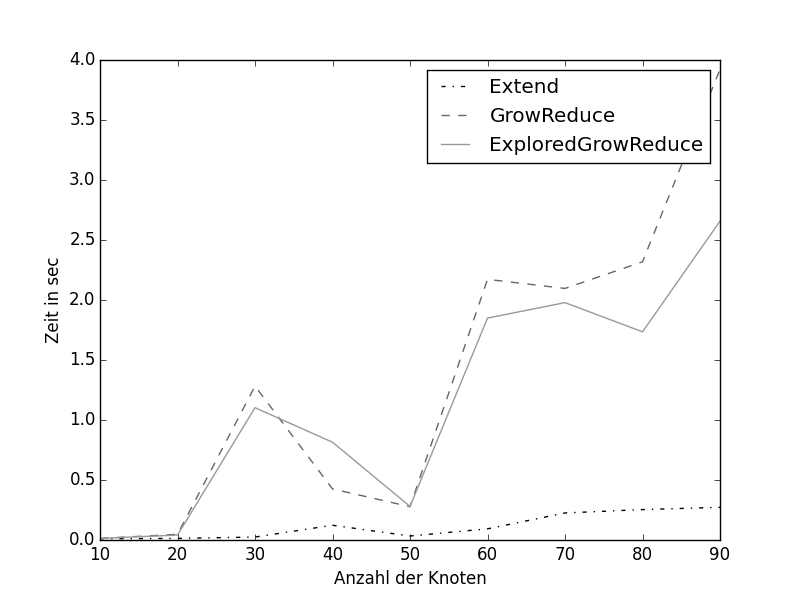
\includegraphics[scale=0.37]{plots/time_node.png}
       \caption{Knotenanzahl-Zeit-Diagramm}
    \end{subfigure}
  \end{tabular}
  \caption{Durchschnittliche Laufzeit von Extend, GrowReduce und ExploredGrowReduce auf dem \vars{
  duplication\_divergence}-Datensatz für Splitcluster}
  \label{fig:time}
\end{figure}



\subsection{Sortierungsverfahren}
In der Tabelle \ref{tab:sort} ist zu sehen, dass die Wahl der Sortierfunktion relevant ist für die Lösungsgröße. Es wurden 4 Datensätze ausgewählt, um zu zeigen, dass die Sortierfunktion erheblichen Einfluss hat und dies hängt auch von dem \cursive{F} und dem Datensatz ab. 
So ist zu erkennen, dass auf dem \vars{bio2}-Datensatz bei unterschiedlichen Sortierfunktionen am besten sind. So ist bei Split-Cluster-Graphen die Hits-Sortierfunktion die Beste und bei Split-Graphen die absteigende Nachbar-Sortierfunktion die Beste.
Auch ist die beste Sortierungsfunktion abhängig vom Datensatz, auf dem \vars{bio1} ist die absteigende Nachbar-Funtion und auf dem \vars{bio2} die aufsteigende Hits-Funktion.
Auch ist interessant, dass bei ($X_{172}$, Triangle), die Random-Funktion und die auf- und absteigenden Nachbar-Funktionen ähnlich schlecht sind, während Hits-Funktionen sowohl absteigend als auch aufsteigend weitaus besser sind.
Hinzufügen ist hier aber, dass die Hits Sortierungsfunktionen erheblich langsamer sind.
Diese Zusammenhänge würde sich lohnen genauer zu untersuchen, waren jedoch im Umfang dieser Arbeit nicht möglich. 
\begin{table}
\centering
\small
\begin{tabular}{cc|ccccc}
\cursive{F} & Datensatz & R & N ASC & N DESC & H ASC & H DESC   \\ 
\hline 
Splitcluster & \vars{bio2} & 37,5 & 34,0 & 28,7 & \textbf{26,6} & 44,6 \\
($2K_2$, $C_4$, $C_5$) & \vars{bio2} & 50,2 & 67,1 & \textbf{32,8} & 45,0 & 55,8 \\
Splitcluster & \vars{bio1} & 87,6 & 85,8 & \textbf{40,7} & 67,4 & 93,2 \\
($X_{172}$, Triangle) & \vars{barabasi} & 234,0 & 232,4 & 237,2 & 157,5 & \textbf{154,3} \\
\end{tabular} 
\caption{Durchschnittliche Größe der Lösung beim ExploredGrowReduce in Abhängigkeit von der Sortierungsfunktion. Dabei steht R für die zufällige Sortierung, N die Sortierung nach der Anzahl der Kanten, H die Sortierung nach der Anzahl von verbotenen Teilgraphen. ASC steht für aufsteiegend und DESC für absteigend. }
\label{tab:sort}
\end{table}


\subsection{Vergleich mit anderen Heuristiken}
In diesem Abschnitt, wird ExploredGrowReduce mit zwei verschiedenen speziellen Heuristiken verglichen. Zuerst wird mit einer Heuristik für das \textsc{Cluster Editing} verglichen und dann mit einer Heuristik für das \textsc{Quasi-Threshold Editing}.

\label{sec:compare}

\subsubsection{Cluster-Editing}
Die 2K-Heuristik basiert auf einem Kernel für das Cluster-Editing-Problem, welches maximal 2K Knoten liefert \cite{Chen12}. Wenn man dort eine Bedingung für die Reduktionsregel abschwächt, kommt eine gute Heuristik für das Cluster-Editing-Problem heraus. Dabei wird die Bedingung mit jedem Durchlauf abgeschwächt. Dabei wurde ein gewichteter Graph verwendet, bei dem es möglich ist zwei Knoten zu vereinigen und durch die entsprechende Anpassung der Gewichte die Strukturinformation beizubehalten. 
Das Vorgehen ist in dem Algorithmus \ref{algo:2k} zu sehen.
Für einen Knoten  $u$ sind folgende Funktionen definiert, wobei $w({u,v})$ die Gewichtung der Kante $(u,v)$ in dem Graphen ist:\\ 

\begin{equation}
costClique(u) = \sum_{\{a,b\} | a \in N^{*}(u), b \in N^{*}(u), \{a,b\} \notin E(G)} |\,w(\{a,b\})\,|
\end{equation}

\begin{equation}
costCut(u) = \sum_{\{a,b\} | a \in N^{*}(u), b \notin N^{*}(u), \{a,b\} \in E(G)} w(\{a,b\})
\end{equation}

\begin{algorithm}
  \captionof{algorithm}{2K-Heuristik}
    \label{algo:2k}
\begin{algorithmic}[1]
\Function{solve2K}{$G$}
\State{\vars{x} $\gets$ 1,0} 
\While{$G$ has a P3}
	\For{each knoten \vars{u} $\in$ E($G$)}
		\If{$2 \cdot x \cdot costClique(u) + x \cdot costCut(u) < |N(u)|)$}
			\For{each $\{a,b\}$  mit $a \in N(u)$, $b \in N(u) \land a \neq b$}
				\State{\func{merge}(a,b)}
			\EndFor
		\EndIf
	\EndFor
	\State{$\vars{x} \gets$ $0,99 \cdot \vars{x} - 0,01$}
\EndWhile

\Return{$G$}
\EndFunction
\end{algorithmic}
\end{algorithm}

In der Tabelle \ref{tab:size_2k} wird die Lösungsgröße zwischen dem 2K-Algorithmus und dem ExploredGrowReduce verglichen. Zu sehen ist, dass der 2K-Algorithmus auf den realen Daten signifikant besser ist. 

\begin{table}
\begin{tabular}{c|c c|c c} 
& \multicolumn{2}{c|}{2K} & \multicolumn{2}{c}{ExploredGrowReduce\footnote{Siehe Algorithmus \ref{algo:ExploredGrowReduce} mit 5 Iterationen }} \\ 
Datensatz & \multicolumn{1}{c}{mean}  &  \multicolumn{1}{c|}{std} &  \multicolumn{1}{c}{mean} &  \multicolumn{1}{c}{std} \\ 
\hline 
bio1  & \textbf{43.44}  & 79.81 & 133.59 & 249,62 \\ 
bio2 & \textbf{34.11} & 19.79 & 113.81 & 166,01 \\ 
duplication-divergence & 155.17 & 217.38 & \textbf{92.30} & 115,22 \\ 
newman-watts-strogatz  & 165.22 & 149,86 & \textbf{152.34} & 127,51 \\ 
albert-barabasi & 324.30 & 316,32 & \textbf{248.84} & 226,87 \\ 
binomial & \textbf{493.17} & 545,19 & 554.61 & 670,91 \\ 

\end{tabular} 
\caption{Vergleich der durchschnittlichen Lösungsgröße}
\label{tab:size_2k}
\end{table}


\subsubsection{\textsc{Quasi-Threshold Editing}}


In \cite{BrandesHSW15} wurde ein neuer schneller und auch für große Graphen geeigneter Algorithmus entwickelt für das \textsc{Quasi-Threshold Edge Editing} Problem. Quasi-Threshold Graphen, auch bekannt als trivial-perfekte Graphen. Diese lassen sich auch als $(P_4, C_4)$-freie Graphen charakterisieren. 

In Tabelle \ref{tab:qual_mover} wird die Lösungsqualität von dem Quasi-Threshold-Mover und unserem Algorithmus ExploredGrowReduce verglichen. Da für den Vergleich der Lösungsqualität die minimale Distanz zum \cursive{F}-freien Graphen bekannt sein muss, wird in der Tabelle \ref{tab:size_mover}  die durchschnittliche Größe der Lösungen verglichen, um auszuschließen, dass der Quasi-Threshold-Mover nur auf den einfachen Instanzen besser ist.
Zu sehen ist, dass der der Quasi-Threshold-Mover um 70\% konsistent besser löst.


\begin{center}
\captionof{table}{Vergleich der durchschnittlichen Lösungsqualität}
\label{tab:qual_mover}
\begin{tabular}{c|c c|c c}
& \multicolumn{2}{c|}{ExploredGrowReduce\footnote{Siehe Algorithmus \ref{algo:ExploredGrowReduce} mit Standard-Parametern }} & \multicolumn{2}{c}{Quasi-Threshold-Mover} \\ 
Datensatz & \multicolumn{1}{c}{mean}  &  \multicolumn{1}{c|}{std} &  \multicolumn{1}{c}{mean} &  \multicolumn{1}{c}{std} \\ 
\hline 
bio1                    & 1,61x     & 1,30  & \textbf{1,05x}    & 0,14 \\ 
bio2                    & 1,69x     & 1,03  & \textbf{1,05x}    & 0,10 \\ 
duplication-divergence  & 1,42x     & 0,33  & \textbf{1,04x}    & 0,05 \\ 
newman-watts-strogatz   & 1,38x     & 0,22  & \textbf{1,06x}    & 0,05 \\ 

\end{tabular} 
\end{center}

\begin{center}
\captionof{table}{Vergleich der durchschnittlichen Lösungsgröße}
\label{tab:size_mover}
\begin{tabular}{c|c c|c c}
 & \multicolumn{2}{c|}{\textbf{ExploredGrowReduce}} & \multicolumn{2}{c}{\textbf{Quasi-Threshold-Mover}} \\ 
Datensatz & \multicolumn{1}{c}{mean}  &  \multicolumn{1}{c|}{std} &  \multicolumn{1}{c}{mean} &  \multicolumn{1}{c}{std} \\ 
\hline 
bio1 & 52.25  & 150.25 & \textbf{20.88} & 46.51 \\ 
bio2 & 23.12 & 19.91 & \textbf{13.89} & 9.64 \\ 
duplication-divergence & 73.87 & 117.35 & \textbf{51.46} & 80.23 \\ 
newman-watts-strogatz & 146.48 & 128.42 & \textbf{103.38} & 87.99 \\ 

\end{tabular} 
\end{center}


\begin{table}
\centering
\begin{tabular}{c cc}
Graph & \textbf{ExploredGrowReduce} & \textbf{Quasi-Threshold-Mover} \\ 
\hline 
\vars{karate} & 26 & 21 \\
\vars{polbooks} & 363 & 226 \\
\vars{power} & 5071 & 2806 \\
\vars{football} & 372 & 259 \\
\vars{lesmiserables} & 147 & 60 \\
\vars{adjnoun} & 391 & 283\\
\vars{celegansneural} & 2035 & 1499 \\
\vars{dolphins} & 103 & 73 \\
\vars{polblogs} & - & 12607 \\
\end{tabular} 
\caption{Vergleich von der Lösungsgröße auf dem Datensatz \vars{UCINetworkDataRepository}}
\label{tab:uci}
\end{table}


\section{Zusammenfassung}\\
In dieser Arbeit wurde gezeigt, dass es möglich ist, gute Heuristiken für \textsc{\cursive{F}-Free Edge Editing} zu finden. Dafür wurden 3 Ansätze entwickelt. Der Forward-Ansatz modifiziert den Graphen so lange bis er \cursive{F}-frei ist. Der Backward-Ansatz baut den Graphen aus einem leeren Graphen auf, bis er möglichst nahe an dem Eingabegraphen ist und dabei \cursive{F}-frei bleibt. Der Grow-Reduce-Ansatz kombiniert diese beiden Ansatz und baut iterativ den Graphen auf und dann modifiziert ihn durch lokale Suche, sodass er \cursive{F}-frei wird. Der Forward-Ansatz zeichnet sich durch gute Lösungen für kleine Graphen aus, während der Backward-Ansatz sich durch eine schnelle Laufzeit auszeichnet. Die besten Lösungen liefern aber der ExploreGrowReduce-Algorithmus, ist jedoch auf großen Graphen nicht sehr schnell.
Der Vergleich mit anderen Heuristiken hat ergeben, dass die speziellen Heuristiken bessere Ergebnisse liefern, aber diese Lösungen durchschnittlich nur um 70\% besser sind.



\subsection{Ausblick}

\textbf{Besser Sortierung von Grow-Reduce}\\
Ein wichtiges Detail bei der Qualität der Lösungen von GrowReduce und ExploredGrowReduce ist die Sortierungsfunktion der Knoten am Anfang. In dieser Arbeit wurden drei sehr einfache Sortierungsfunktionen verwendet. Man könnte untersuchen, ob es bessere allgemeine Sortierfunktionen gibt. Auch wären spezielle Sortierungsfunktionen, die vom \cursive{F} abhängen, sehr interessant.\\


\textbf{Obere und untere Schranken}\\
Obere und untere Schranken für die Lösungsqualität zu untersuchen, wäre interessant.\\

\textbf{Heuristiken für Subgraph-Isomorphismen}\\
Da viel Zeit bei der Suche nach den verbotenen Teilgraphen investiert wird, wäre zuerst eine Vereinfachung der Graphens durch das schnelle Lösen mittels der Verwendungen einer Heuristik für die Suche für die Teilgraphen \cite{Dehmer13} optimal. Und dann könnte man mittels einen von diesen hier vorgestellten Algorithmen eine Lösung endgültig bekommen, wo sichergestellt ist, dass der resultierende Graph \cursive{F}-frei ist. Dies hätte vor allem einen Vorteil bei großen Graphen, wo die hier vorgestellten Algorithmen langsam sind.\\

\textbf{Besseres Konvergenzkriterium}\\
In einigen der Algorithmen wurden Konvergenzkriterien verwendet, um zu entscheiden ob eine Änderungen der Kante sinnvoll ist oder nicht. Dies wurde so implementiert, dass die Anzahl der verbotenen Teilgraphen vor und nach der Änderung gezählt wurde, was jedoch sehr zeitaufwändig ist. Man könnte es verbessern, indem man auch hier eine Abschätzung oder eine Heuristik für das Subgraphen-Isomorphismen Problem verwendet.


\newpage
\bibliographystyle{plain}
\bibliography{biblio}

\end{document}
